\chapter{Transformada de \emph{Fourier}}

\section{Integrales de \emph{Fourier}}
\begin{figure}[H]
    \centering
    % GNUPLOT: LaTeX picture with Postscript
\begingroup
  \makeatletter
  \providecommand\color[2][]{%
    \GenericError{(gnuplot) \space\space\space\@spaces}{%
      Package color not loaded in conjunction with
      terminal option `colourtext'%
    }{See the gnuplot documentation for explanation.%
    }{Either use 'blacktext' in gnuplot or load the package
      color.sty in LaTeX.}%
    \renewcommand\color[2][]{}%
  }%
  \providecommand\includegraphics[2][]{%
    \GenericError{(gnuplot) \space\space\space\@spaces}{%
      Package graphicx or graphics not loaded%
    }{See the gnuplot documentation for explanation.%
    }{The gnuplot epslatex terminal needs graphicx.sty or graphics.sty.}%
    \renewcommand\includegraphics[2][]{}%
  }%
  \providecommand\rotatebox[2]{#2}%
  \@ifundefined{ifGPcolor}{%
    \newif\ifGPcolor
    \GPcolorfalse
  }{}%
  \@ifundefined{ifGPblacktext}{%
    \newif\ifGPblacktext
    \GPblacktexttrue
  }{}%
  % define a \g@addto@macro without @ in the name:
  \let\gplgaddtomacro\g@addto@macro
  % define empty templates for all commands taking text:
  \gdef\gplbacktext{}%
  \gdef\gplfronttext{}%
  \makeatother
  \ifGPblacktext
    % no textcolor at all
    \def\colorrgb#1{}%
    \def\colorgray#1{}%
  \else
    % gray or color?
    \ifGPcolor
      \def\colorrgb#1{\color[rgb]{#1}}%
      \def\colorgray#1{\color[gray]{#1}}%
      \expandafter\def\csname LTw\endcsname{\color{white}}%
      \expandafter\def\csname LTb\endcsname{\color{black}}%
      \expandafter\def\csname LTa\endcsname{\color{black}}%
      \expandafter\def\csname LT0\endcsname{\color[rgb]{1,0,0}}%
      \expandafter\def\csname LT1\endcsname{\color[rgb]{0,1,0}}%
      \expandafter\def\csname LT2\endcsname{\color[rgb]{0,0,1}}%
      \expandafter\def\csname LT3\endcsname{\color[rgb]{1,0,1}}%
      \expandafter\def\csname LT4\endcsname{\color[rgb]{0,1,1}}%
      \expandafter\def\csname LT5\endcsname{\color[rgb]{1,1,0}}%
      \expandafter\def\csname LT6\endcsname{\color[rgb]{0,0,0}}%
      \expandafter\def\csname LT7\endcsname{\color[rgb]{1,0.3,0}}%
      \expandafter\def\csname LT8\endcsname{\color[rgb]{0.5,0.5,0.5}}%
    \else
      % gray
      \def\colorrgb#1{\color{black}}%
      \def\colorgray#1{\color[gray]{#1}}%
      \expandafter\def\csname LTw\endcsname{\color{white}}%
      \expandafter\def\csname LTb\endcsname{\color{black}}%
      \expandafter\def\csname LTa\endcsname{\color{black}}%
      \expandafter\def\csname LT0\endcsname{\color{black}}%
      \expandafter\def\csname LT1\endcsname{\color{black}}%
      \expandafter\def\csname LT2\endcsname{\color{black}}%
      \expandafter\def\csname LT3\endcsname{\color{black}}%
      \expandafter\def\csname LT4\endcsname{\color{black}}%
      \expandafter\def\csname LT5\endcsname{\color{black}}%
      \expandafter\def\csname LT6\endcsname{\color{black}}%
      \expandafter\def\csname LT7\endcsname{\color{black}}%
      \expandafter\def\csname LT8\endcsname{\color{black}}%
    \fi
  \fi
    \setlength{\unitlength}{0.0500bp}%
    \ifx\gptboxheight\undefined%
      \newlength{\gptboxheight}%
      \newlength{\gptboxwidth}%
      \newsavebox{\gptboxtext}%
    \fi%
    \setlength{\fboxrule}{0.5pt}%
    \setlength{\fboxsep}{1pt}%
    \definecolor{tbcol}{rgb}{1,1,1}%
\begin{picture}(7200.00,2160.00)%
    \gplgaddtomacro\gplbacktext{%
      \csname LTb\endcsname%%
      \put(3480,192){\makebox(0,0)[r]{\strut{}}}%
      \put(3480,644){\makebox(0,0)[r]{\strut{}}}%
      \put(3480,1096){\makebox(0,0)[r]{\strut{}}}%
      \put(3480,1547){\makebox(0,0)[r]{\strut{}}}%
      \put(3480,1999){\makebox(0,0)[r]{\strut{}}}%
      \put(240,421){\makebox(0,0){\strut{}}}%
      \put(907,421){\makebox(0,0){\strut{}}}%
      \put(1574,421){\makebox(0,0){\strut{}}}%
      \put(2241,421){\makebox(0,0){\strut{}}}%
      \put(2908,421){\makebox(0,0){\strut{}}}%
      \put(3576,421){\makebox(0,0){\strut{}}}%
      \put(4243,421){\makebox(0,0){\strut{}}}%
      \put(4910,421){\makebox(0,0){\strut{}}}%
      \put(5577,421){\makebox(0,0){\strut{}}}%
      \put(6244,421){\makebox(0,0){\strut{}}}%
      \put(6911,421){\makebox(0,0){\strut{}}}%
      \csname LTb\endcsname%%
      \put(7778,644){\makebox(0,0)[l]{\strut{}$t$}}%
      \put(3876,2180){\makebox(0,0)[l]{\strut{}$f(t)$}}%
      \put(574,418){\makebox(0,0)[l]{\strut{}$-2T$}}%
      \put(2041,418){\makebox(0,0)[l]{\strut{}$- T$}}%
      \put(4843,418){\makebox(0,0)[l]{\strut{}$  T$}}%
      \put(6110,418){\makebox(0,0)[l]{\strut{}$ 2T$}}%
    }%
    \gplgaddtomacro\gplfronttext{%
    }%
    \gplgaddtomacro\gplbacktext{%
      \csname LTb\endcsname%%
      \put(3480,192){\makebox(0,0)[r]{\strut{}}}%
      \put(3480,644){\makebox(0,0)[r]{\strut{}}}%
      \put(3480,1096){\makebox(0,0)[r]{\strut{}}}%
      \put(3480,1547){\makebox(0,0)[r]{\strut{}}}%
      \put(3480,1999){\makebox(0,0)[r]{\strut{}}}%
      \put(240,421){\makebox(0,0){\strut{}}}%
      \put(907,421){\makebox(0,0){\strut{}}}%
      \put(1574,421){\makebox(0,0){\strut{}}}%
      \put(2241,421){\makebox(0,0){\strut{}}}%
      \put(2908,421){\makebox(0,0){\strut{}}}%
      \put(3576,421){\makebox(0,0){\strut{}}}%
      \put(4243,421){\makebox(0,0){\strut{}}}%
      \put(4910,421){\makebox(0,0){\strut{}}}%
      \put(5577,421){\makebox(0,0){\strut{}}}%
      \put(6244,421){\makebox(0,0){\strut{}}}%
      \put(6911,421){\makebox(0,0){\strut{}}}%
      \csname LTb\endcsname%%
      \put(7778,644){\makebox(0,0)[l]{\strut{}$t$}}%
      \put(3876,2180){\makebox(0,0)[l]{\strut{}$f(t)$}}%
      \put(574,418){\makebox(0,0)[l]{\strut{}$-2T$}}%
      \put(2041,418){\makebox(0,0)[l]{\strut{}$- T$}}%
      \put(4843,418){\makebox(0,0)[l]{\strut{}$  T$}}%
      \put(6110,418){\makebox(0,0)[l]{\strut{}$ 2T$}}%
    }%
    \gplgaddtomacro\gplfronttext{%
    }%
    \gplgaddtomacro\gplbacktext{%
      \csname LTb\endcsname%%
      \put(3480,192){\makebox(0,0)[r]{\strut{}}}%
      \put(3480,644){\makebox(0,0)[r]{\strut{}}}%
      \put(3480,1096){\makebox(0,0)[r]{\strut{}}}%
      \put(3480,1547){\makebox(0,0)[r]{\strut{}}}%
      \put(3480,1999){\makebox(0,0)[r]{\strut{}}}%
      \put(240,421){\makebox(0,0){\strut{}}}%
      \put(907,421){\makebox(0,0){\strut{}}}%
      \put(1574,421){\makebox(0,0){\strut{}}}%
      \put(2241,421){\makebox(0,0){\strut{}}}%
      \put(2908,421){\makebox(0,0){\strut{}}}%
      \put(3576,421){\makebox(0,0){\strut{}}}%
      \put(4243,421){\makebox(0,0){\strut{}}}%
      \put(4910,421){\makebox(0,0){\strut{}}}%
      \put(5577,421){\makebox(0,0){\strut{}}}%
      \put(6244,421){\makebox(0,0){\strut{}}}%
      \put(6911,421){\makebox(0,0){\strut{}}}%
      \csname LTb\endcsname%%
      \put(7778,644){\makebox(0,0)[l]{\strut{}$t$}}%
      \put(3876,2180){\makebox(0,0)[l]{\strut{}$f(t)$}}%
      \put(574,418){\makebox(0,0)[l]{\strut{}$-2T$}}%
      \put(2041,418){\makebox(0,0)[l]{\strut{}$- T$}}%
      \put(4843,418){\makebox(0,0)[l]{\strut{}$  T$}}%
      \put(6110,418){\makebox(0,0)[l]{\strut{}$ 2T$}}%
    }%
    \gplgaddtomacro\gplfronttext{%
    }%
    \gplgaddtomacro\gplbacktext{%
      \csname LTb\endcsname%%
      \put(3480,192){\makebox(0,0)[r]{\strut{}}}%
      \put(3480,644){\makebox(0,0)[r]{\strut{}}}%
      \put(3480,1096){\makebox(0,0)[r]{\strut{}}}%
      \put(3480,1547){\makebox(0,0)[r]{\strut{}}}%
      \put(3480,1999){\makebox(0,0)[r]{\strut{}}}%
      \put(240,421){\makebox(0,0){\strut{}}}%
      \put(907,421){\makebox(0,0){\strut{}}}%
      \put(1574,421){\makebox(0,0){\strut{}}}%
      \put(2241,421){\makebox(0,0){\strut{}}}%
      \put(2908,421){\makebox(0,0){\strut{}}}%
      \put(3576,421){\makebox(0,0){\strut{}}}%
      \put(4243,421){\makebox(0,0){\strut{}}}%
      \put(4910,421){\makebox(0,0){\strut{}}}%
      \put(5577,421){\makebox(0,0){\strut{}}}%
      \put(6244,421){\makebox(0,0){\strut{}}}%
      \put(6911,421){\makebox(0,0){\strut{}}}%
      \csname LTb\endcsname%%
      \put(7778,644){\makebox(0,0)[l]{\strut{}$t$}}%
      \put(3876,2180){\makebox(0,0)[l]{\strut{}$f(t)$}}%
      \put(574,418){\makebox(0,0)[l]{\strut{}$-2T$}}%
      \put(2041,418){\makebox(0,0)[l]{\strut{}$- T$}}%
      \put(4843,418){\makebox(0,0)[l]{\strut{}$  T$}}%
      \put(6110,418){\makebox(0,0)[l]{\strut{}$ 2T$}}%
    }%
    \gplgaddtomacro\gplfronttext{%
    }%
    \gplgaddtomacro\gplbacktext{%
      \csname LTb\endcsname%%
      \put(3480,192){\makebox(0,0)[r]{\strut{}}}%
      \put(3480,644){\makebox(0,0)[r]{\strut{}}}%
      \put(3480,1096){\makebox(0,0)[r]{\strut{}}}%
      \put(3480,1547){\makebox(0,0)[r]{\strut{}}}%
      \put(3480,1999){\makebox(0,0)[r]{\strut{}}}%
      \put(240,421){\makebox(0,0){\strut{}}}%
      \put(907,421){\makebox(0,0){\strut{}}}%
      \put(1574,421){\makebox(0,0){\strut{}}}%
      \put(2241,421){\makebox(0,0){\strut{}}}%
      \put(2908,421){\makebox(0,0){\strut{}}}%
      \put(3576,421){\makebox(0,0){\strut{}}}%
      \put(4243,421){\makebox(0,0){\strut{}}}%
      \put(4910,421){\makebox(0,0){\strut{}}}%
      \put(5577,421){\makebox(0,0){\strut{}}}%
      \put(6244,421){\makebox(0,0){\strut{}}}%
      \put(6911,421){\makebox(0,0){\strut{}}}%
      \csname LTb\endcsname%%
      \put(7778,644){\makebox(0,0)[l]{\strut{}$t$}}%
      \put(3876,2180){\makebox(0,0)[l]{\strut{}$f(t)$}}%
      \put(574,418){\makebox(0,0)[l]{\strut{}$-2T$}}%
      \put(2041,418){\makebox(0,0)[l]{\strut{}$- T$}}%
      \put(4843,418){\makebox(0,0)[l]{\strut{}$  T$}}%
      \put(6110,418){\makebox(0,0)[l]{\strut{}$ 2T$}}%
    }%
    \gplgaddtomacro\gplfronttext{%
    }%
    \gplbacktext
    \put(0,0){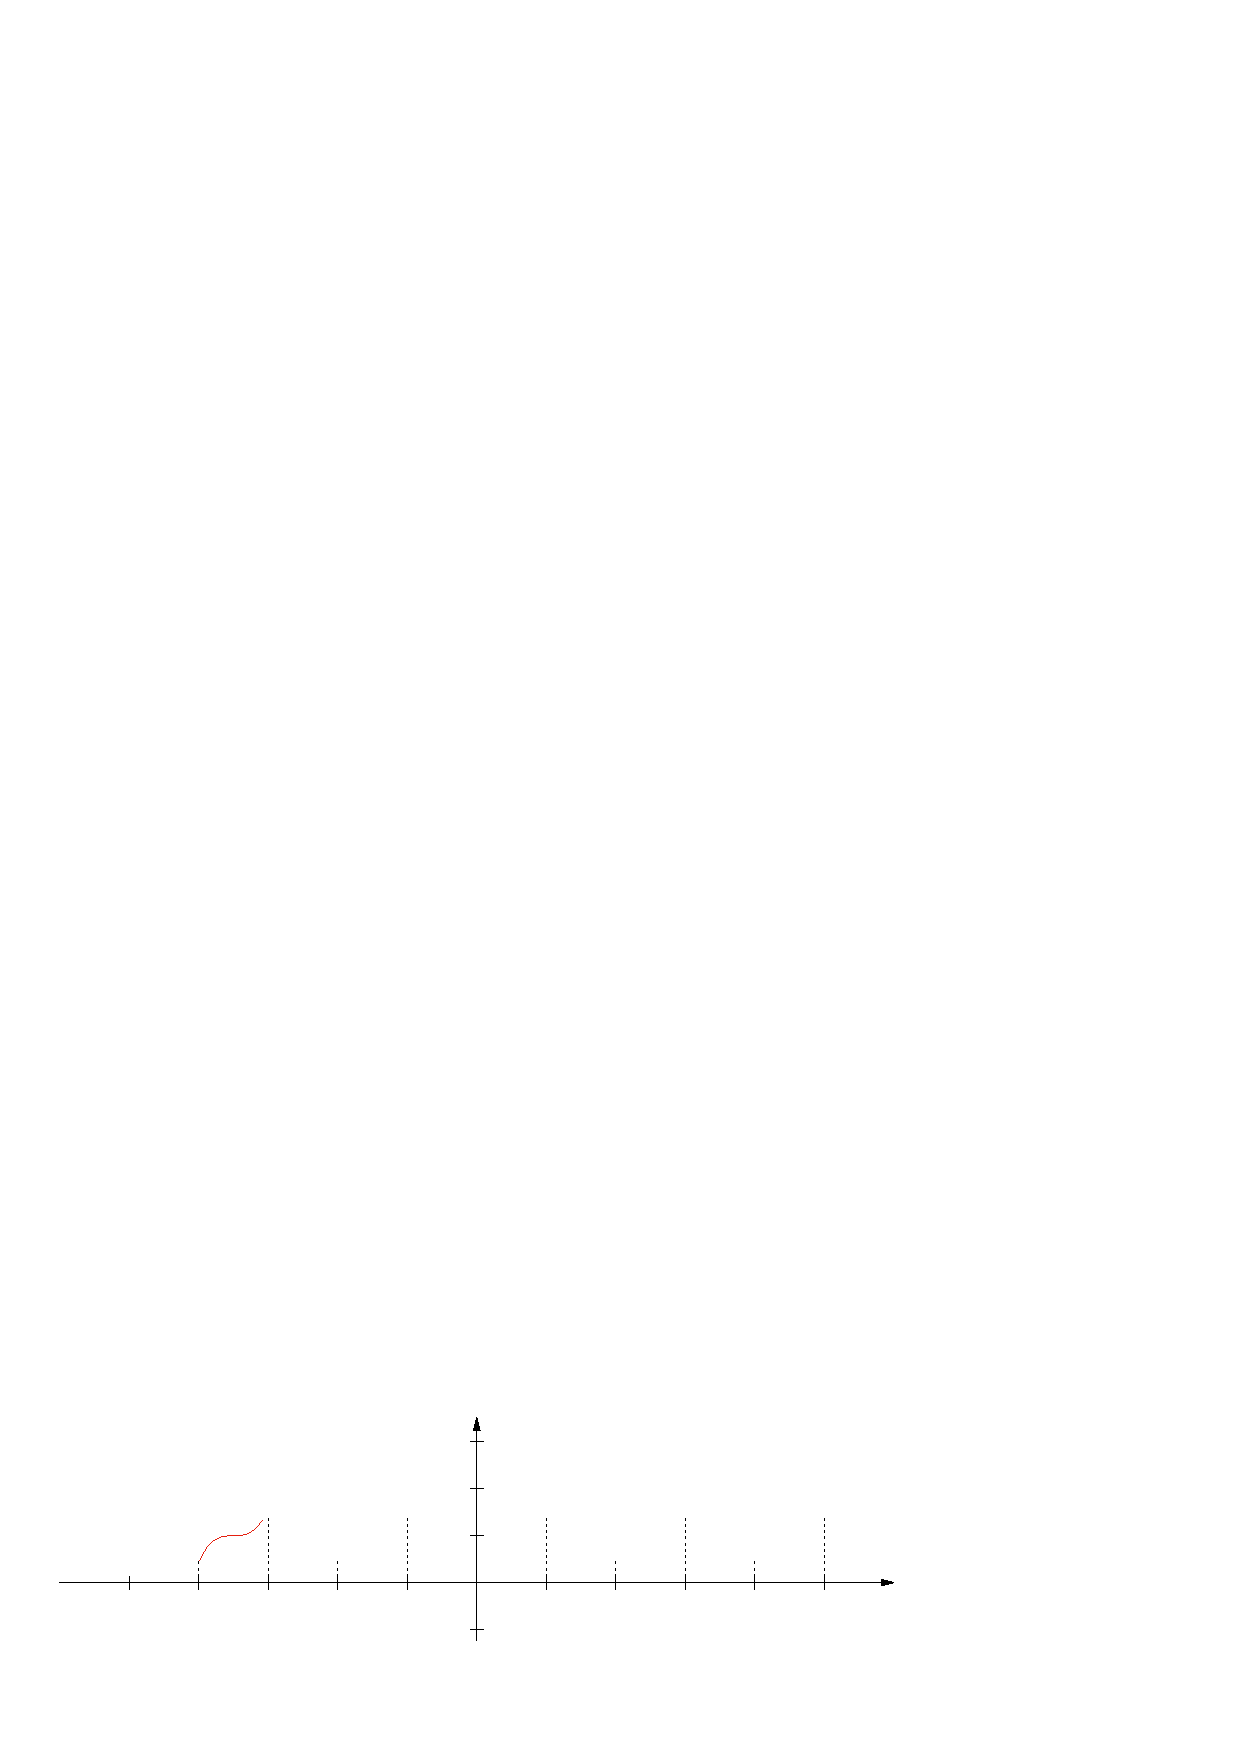
\includegraphics[width={360.00bp},height={108.00bp}]{figura_04_01}}%
    \gplfronttext
  \end{picture}%
\endgroup

\end{figure}

Cuando $f(t)$ es periódica tiene la siguiente representación (forma compleja):
\begin{equation*}
    f(t)=\sum_{n=-\infty}^\infty\,c_n\,e^{jn\omega_0\,t}
\end{equation*}

Donde:
\begin{equation*}
    c_n=\frac{1}{T}\int_{-T/2}^{T/2}\,f(t)\,e^{-jn\omega_0\,t}\,dt
\end{equation*}

Si $T\to\infty$, entonces $\omega_0\to0$, y la función deja de ser periódica.
\begin{equation*}
    f(t)=\sum_{n=-\infty}^\infty\left[
        \frac{1}{T}\int_{-T/2}^{T/2}\,f(\tau)\,e^{-jn\omega_0\,\tau}\,d\tau
    \right]\,e^{jn\omega_0\,t}
\end{equation*}
\begin{equation*}
    \frac{1}{T}=\frac{\omega_0}{2\pi}
\end{equation*}
\begin{equation*}
    f(t)=\frac{1}{2\pi}\sum_{n=-\infty}^\infty\left[
        \int_{-T/2}^{T/2}\,f(\tau)\,e^{-jn\omega_0\,\tau}\,d\tau
    \right]\,e^{jn\omega_0\,t}\,\omega_0
\end{equation*}
\begin{equation*}
    \omega_0=d\omega
\end{equation*}
\begin{equation*}
    n\omega_0=\omega
\end{equation*}
\begin{equation}
    f(t)=\frac{1}{2\pi}\int_{-\infty}^\infty\left[
        \int_{-\infty}^{\infty}\,f(\tau)\,e^{-j\omega\tau}\,d\tau
    \right]\,e^{j\omega\,t}\,d\omega
\end{equation}

Se define como transformada de \emph{Fourier}:
\begin{equation}
    F(\omega)=\int_{-\infty}^{\infty}\,f(t)\,e^{-j\omega\,t}\,dt
\end{equation}

Se define como transformada inversa de \emph{Fourier}:
\begin{equation}
    f(t)=\frac{1}{2\pi}\int_{-\infty}^\infty\,F(\omega)\,e^{j\omega\,t}\,d\omega
\end{equation}

\section{Transformada de \emph{Fourier}}
Dada una función $f(t)$ se define la transformada de \emph{Fourier}:
\begin{equation}
    \mathcal{F}\{f(t)\}=F(\omega)
        =\int_{-\infty}^{\infty}f(t)\,e^{-j\omega\,t}\,dt
\end{equation}

Donde: $f(t)$ es una función no periódica.

La transformada de \emph{Fourier} convierte una función del dominio del tiempo
($t$) al dominio de la frecuencia ($\omega$) la cual será una variable continua.

Para $f(t)\in\mathbb{R}$:
\begin{equation*}
\begin{split}
    F(\omega)
        &=\int_{-\infty}^{\infty}f(t)\,e^{-j\omega\,t}\,dt\\
        &=\int_{-\infty}^{\infty}f(t)[\cos(\omega\,t)-j\sen(\omega\,t)]\,dt\\
        &=\int_{-\infty}^{\infty}f(t)\cos(\omega\,t)\,dt
            -j\int_{-\infty}^{\infty}f(t)\sen(\omega\,t)\,dt\\
        &=R(\omega)+jX(\omega)\\
\end{split}
\end{equation*}
\begin{equation*}
    R(\omega)=\int_{-\infty}^{\infty}f(t)\cos(\omega\,t)\,dt
\end{equation*}
\begin{equation*}
    X(\omega)=-\int_{-\infty}^{\infty}f(t)\sen(\omega\,t)\,dt\\
\end{equation*}

La parte real $R(\omega)$ es una función par:
\begin{equation*}
    R(-\omega)=R(\omega)
\end{equation*}

La parte imaginaria $X(\omega)$ es una función impar:
\begin{equation*}
    X(-\omega)=-X(\omega)
\end{equation*}

Por tanto:

Si $f(t)$ es par, entonces $X(\omega)=0$.

Si $f(t)$ es impar, entonces $R(\omega)=0$.

\section{Espectros continuos de frecuencia}
\begin{equation*}
    F(\omega)=R(\omega)+jX(\omega)
\end{equation*}

Modulo:
\begin{equation*}
    |F(\omega)|=\sqrt{R^2(\omega)+X^2(\omega)}
\end{equation*}

Argumento:
\begin{equation*}
    \theta(\omega)=\arctan\left(\frac{X(\omega)}{R(\omega)}\right)
\end{equation*}

\textbf{Ejemplo 1:} Hallar $F(\omega)$ de la función y graficar los espectros.
\begin{equation*}
    f(t)=u(t+a)-u(t-a)
\end{equation*}
\begin{figure}[H]
    \centering
    % GNUPLOT: LaTeX picture with Postscript
\begingroup
  \makeatletter
  \providecommand\color[2][]{%
    \GenericError{(gnuplot) \space\space\space\@spaces}{%
      Package color not loaded in conjunction with
      terminal option `colourtext'%
    }{See the gnuplot documentation for explanation.%
    }{Either use 'blacktext' in gnuplot or load the package
      color.sty in LaTeX.}%
    \renewcommand\color[2][]{}%
  }%
  \providecommand\includegraphics[2][]{%
    \GenericError{(gnuplot) \space\space\space\@spaces}{%
      Package graphicx or graphics not loaded%
    }{See the gnuplot documentation for explanation.%
    }{The gnuplot epslatex terminal needs graphicx.sty or graphics.sty.}%
    \renewcommand\includegraphics[2][]{}%
  }%
  \providecommand\rotatebox[2]{#2}%
  \@ifundefined{ifGPcolor}{%
    \newif\ifGPcolor
    \GPcolorfalse
  }{}%
  \@ifundefined{ifGPblacktext}{%
    \newif\ifGPblacktext
    \GPblacktexttrue
  }{}%
  % define a \g@addto@macro without @ in the name:
  \let\gplgaddtomacro\g@addto@macro
  % define empty templates for all commands taking text:
  \gdef\gplbacktext{}%
  \gdef\gplfronttext{}%
  \makeatother
  \ifGPblacktext
    % no textcolor at all
    \def\colorrgb#1{}%
    \def\colorgray#1{}%
  \else
    % gray or color?
    \ifGPcolor
      \def\colorrgb#1{\color[rgb]{#1}}%
      \def\colorgray#1{\color[gray]{#1}}%
      \expandafter\def\csname LTw\endcsname{\color{white}}%
      \expandafter\def\csname LTb\endcsname{\color{black}}%
      \expandafter\def\csname LTa\endcsname{\color{black}}%
      \expandafter\def\csname LT0\endcsname{\color[rgb]{1,0,0}}%
      \expandafter\def\csname LT1\endcsname{\color[rgb]{0,1,0}}%
      \expandafter\def\csname LT2\endcsname{\color[rgb]{0,0,1}}%
      \expandafter\def\csname LT3\endcsname{\color[rgb]{1,0,1}}%
      \expandafter\def\csname LT4\endcsname{\color[rgb]{0,1,1}}%
      \expandafter\def\csname LT5\endcsname{\color[rgb]{1,1,0}}%
      \expandafter\def\csname LT6\endcsname{\color[rgb]{0,0,0}}%
      \expandafter\def\csname LT7\endcsname{\color[rgb]{1,0.3,0}}%
      \expandafter\def\csname LT8\endcsname{\color[rgb]{0.5,0.5,0.5}}%
    \else
      % gray
      \def\colorrgb#1{\color{black}}%
      \def\colorgray#1{\color[gray]{#1}}%
      \expandafter\def\csname LTw\endcsname{\color{white}}%
      \expandafter\def\csname LTb\endcsname{\color{black}}%
      \expandafter\def\csname LTa\endcsname{\color{black}}%
      \expandafter\def\csname LT0\endcsname{\color{black}}%
      \expandafter\def\csname LT1\endcsname{\color{black}}%
      \expandafter\def\csname LT2\endcsname{\color{black}}%
      \expandafter\def\csname LT3\endcsname{\color{black}}%
      \expandafter\def\csname LT4\endcsname{\color{black}}%
      \expandafter\def\csname LT5\endcsname{\color{black}}%
      \expandafter\def\csname LT6\endcsname{\color{black}}%
      \expandafter\def\csname LT7\endcsname{\color{black}}%
      \expandafter\def\csname LT8\endcsname{\color{black}}%
    \fi
  \fi
    \setlength{\unitlength}{0.0500bp}%
    \ifx\gptboxheight\undefined%
      \newlength{\gptboxheight}%
      \newlength{\gptboxwidth}%
      \newsavebox{\gptboxtext}%
    \fi%
    \setlength{\fboxrule}{0.5pt}%
    \setlength{\fboxsep}{1pt}%
    \definecolor{tbcol}{rgb}{1,1,1}%
\begin{picture}(2160.00,1728.00)%
    \gplgaddtomacro\gplbacktext{%
      \csname LTb\endcsname%%
      \put(960,192){\makebox(0,0)[r]{\strut{}}}%
      \put(960,650){\makebox(0,0)[r]{\strut{}}}%
      \put(960,1109){\makebox(0,0)[r]{\strut{}}}%
      \put(960,1567){\makebox(0,0)[r]{\strut{}}}%
      \put(240,427){\makebox(0,0){\strut{}}}%
      \put(648,427){\makebox(0,0){\strut{}}}%
      \put(1056,427){\makebox(0,0){\strut{}}}%
      \put(1463,427){\makebox(0,0){\strut{}}}%
      \put(1871,427){\makebox(0,0){\strut{}}}%
      \csname LTb\endcsname%%
      \put(2279,650){\makebox(0,0)[l]{\strut{}$t$}}%
      \put(1239,1750){\makebox(0,0)[l]{\strut{}$f(t)$}}%
      \put(1422,375){\makebox(0,0)[l]{\strut{}$ a$}}%
      \put(444,375){\makebox(0,0)[l]{\strut{}$-a$}}%
      \put(852,1292){\makebox(0,0)[l]{\strut{}$1$}}%
    }%
    \gplgaddtomacro\gplfronttext{%
    }%
    \gplbacktext
    \put(0,0){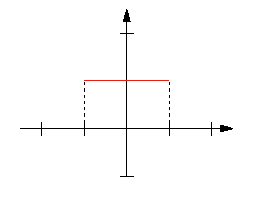
\includegraphics[width={108.00bp},height={86.40bp}]{figura_04_02}}%
    \gplfronttext
  \end{picture}%
\endgroup

\end{figure}
\begin{equation*}
\begin{split}
    F(\omega)
        &=\int_{-a}^a\,1\,e^{-j\omega\,t}\,dt\\
        &=\frac{e^{-j\omega\,t}}{-j\omega}\Biggr|_{-a}^a\\
        &=\frac{e^{-ja\omega}-e^{ja\omega}}{-j\omega}\\
        &=\frac{-2j\sen(a\omega)}{-j\omega}\\
        &=\frac{2\sen(a\omega)}{\omega}\\
\end{split}
\end{equation*}
\begin{equation}
    \mathcal{F}\{u(t+a)-u(t-a)\}=\frac{2\sen(a\omega)}{\omega}
\end{equation}
\begin{equation*}
    |F(\omega)|=\Big|\frac{2\sen(a\omega)}{\omega}\Big|
\end{equation*}

Para $\omega=0$, existe una discontinuidad:
\begin{equation*}
    \lim_{\omega\to0}\left(\frac{2\sen(a\omega)}{\omega}\right)=2a
\end{equation*}
\begin{figure}[H]
    \centering
    \begin{minipage}{.4\textwidth}
        \centering
        % GNUPLOT: LaTeX picture with Postscript
\begingroup
  \makeatletter
  \providecommand\color[2][]{%
    \GenericError{(gnuplot) \space\space\space\@spaces}{%
      Package color not loaded in conjunction with
      terminal option `colourtext'%
    }{See the gnuplot documentation for explanation.%
    }{Either use 'blacktext' in gnuplot or load the package
      color.sty in LaTeX.}%
    \renewcommand\color[2][]{}%
  }%
  \providecommand\includegraphics[2][]{%
    \GenericError{(gnuplot) \space\space\space\@spaces}{%
      Package graphicx or graphics not loaded%
    }{See the gnuplot documentation for explanation.%
    }{The gnuplot epslatex terminal needs graphicx.sty or graphics.sty.}%
    \renewcommand\includegraphics[2][]{}%
  }%
  \providecommand\rotatebox[2]{#2}%
  \@ifundefined{ifGPcolor}{%
    \newif\ifGPcolor
    \GPcolorfalse
  }{}%
  \@ifundefined{ifGPblacktext}{%
    \newif\ifGPblacktext
    \GPblacktexttrue
  }{}%
  % define a \g@addto@macro without @ in the name:
  \let\gplgaddtomacro\g@addto@macro
  % define empty templates for all commands taking text:
  \gdef\gplbacktext{}%
  \gdef\gplfronttext{}%
  \makeatother
  \ifGPblacktext
    % no textcolor at all
    \def\colorrgb#1{}%
    \def\colorgray#1{}%
  \else
    % gray or color?
    \ifGPcolor
      \def\colorrgb#1{\color[rgb]{#1}}%
      \def\colorgray#1{\color[gray]{#1}}%
      \expandafter\def\csname LTw\endcsname{\color{white}}%
      \expandafter\def\csname LTb\endcsname{\color{black}}%
      \expandafter\def\csname LTa\endcsname{\color{black}}%
      \expandafter\def\csname LT0\endcsname{\color[rgb]{1,0,0}}%
      \expandafter\def\csname LT1\endcsname{\color[rgb]{0,1,0}}%
      \expandafter\def\csname LT2\endcsname{\color[rgb]{0,0,1}}%
      \expandafter\def\csname LT3\endcsname{\color[rgb]{1,0,1}}%
      \expandafter\def\csname LT4\endcsname{\color[rgb]{0,1,1}}%
      \expandafter\def\csname LT5\endcsname{\color[rgb]{1,1,0}}%
      \expandafter\def\csname LT6\endcsname{\color[rgb]{0,0,0}}%
      \expandafter\def\csname LT7\endcsname{\color[rgb]{1,0.3,0}}%
      \expandafter\def\csname LT8\endcsname{\color[rgb]{0.5,0.5,0.5}}%
    \else
      % gray
      \def\colorrgb#1{\color{black}}%
      \def\colorgray#1{\color[gray]{#1}}%
      \expandafter\def\csname LTw\endcsname{\color{white}}%
      \expandafter\def\csname LTb\endcsname{\color{black}}%
      \expandafter\def\csname LTa\endcsname{\color{black}}%
      \expandafter\def\csname LT0\endcsname{\color{black}}%
      \expandafter\def\csname LT1\endcsname{\color{black}}%
      \expandafter\def\csname LT2\endcsname{\color{black}}%
      \expandafter\def\csname LT3\endcsname{\color{black}}%
      \expandafter\def\csname LT4\endcsname{\color{black}}%
      \expandafter\def\csname LT5\endcsname{\color{black}}%
      \expandafter\def\csname LT6\endcsname{\color{black}}%
      \expandafter\def\csname LT7\endcsname{\color{black}}%
      \expandafter\def\csname LT8\endcsname{\color{black}}%
    \fi
  \fi
    \setlength{\unitlength}{0.0500bp}%
    \ifx\gptboxheight\undefined%
      \newlength{\gptboxheight}%
      \newlength{\gptboxwidth}%
      \newsavebox{\gptboxtext}%
    \fi%
    \setlength{\fboxrule}{0.5pt}%
    \setlength{\fboxsep}{1pt}%
    \definecolor{tbcol}{rgb}{1,1,1}%
\begin{picture}(3168.00,2160.00)%
    \gplgaddtomacro\gplbacktext{%
      \csname LTb\endcsname%%
      \put(1464,644){\makebox(0,0)[r]{\strut{}}}%
      \put(1464,1547){\makebox(0,0)[r]{\strut{}}}%
      \put(240,421){\makebox(0,0){\strut{}}}%
      \put(570,421){\makebox(0,0){\strut{}}}%
      \put(900,421){\makebox(0,0){\strut{}}}%
      \put(1230,421){\makebox(0,0){\strut{}}}%
      \put(1560,421){\makebox(0,0){\strut{}}}%
      \put(1889,421){\makebox(0,0){\strut{}}}%
      \put(2219,421){\makebox(0,0){\strut{}}}%
      \put(2549,421){\makebox(0,0){\strut{}}}%
      \put(2879,421){\makebox(0,0){\strut{}}}%
      \csname LTb\endcsname%%
      \put(3110,644){\makebox(0,0)[l]{\strut{}$\omega$}}%
      \put(751,2270){\makebox(0,0)[l]{\strut{}$|F(\omega)|$}}%
    }%
    \gplgaddtomacro\gplfronttext{%
    }%
    \gplbacktext
    \put(0,0){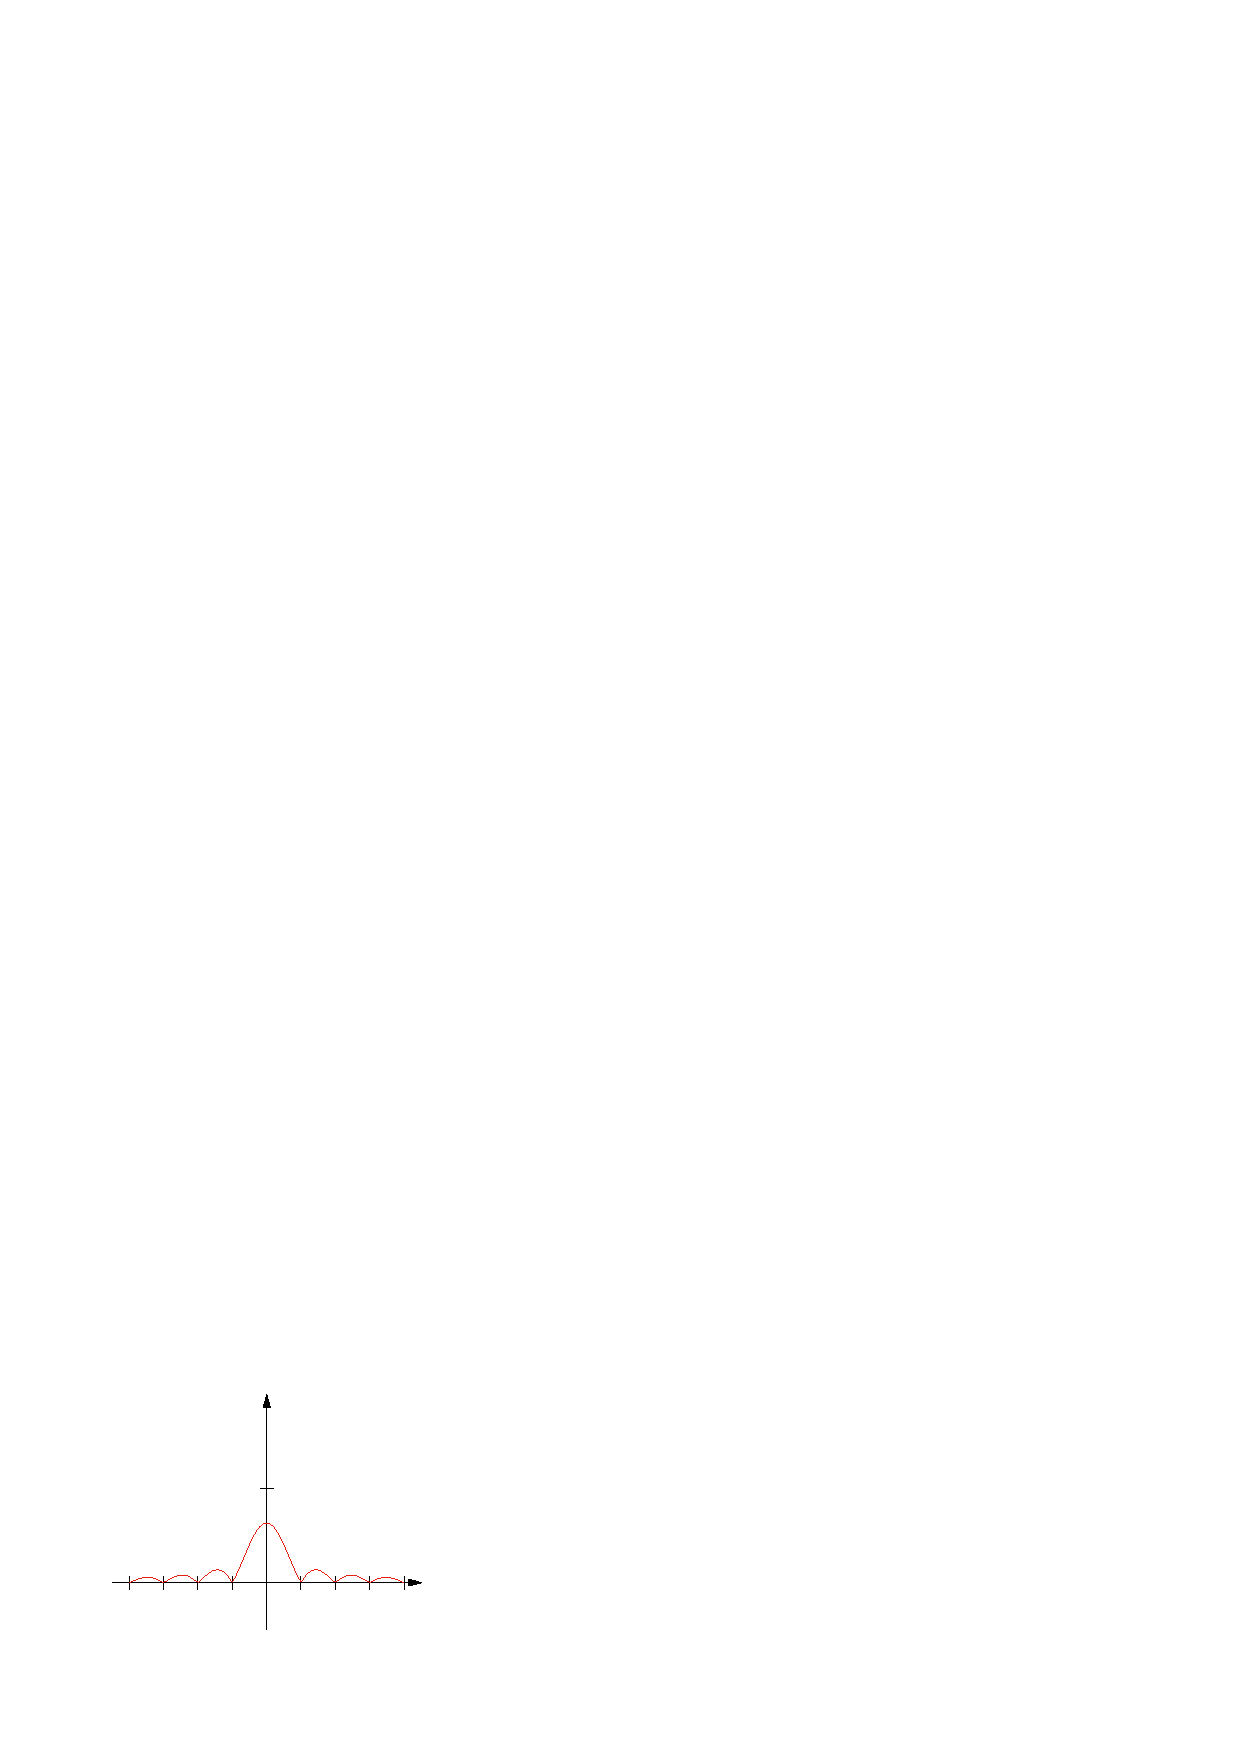
\includegraphics[width={158.40bp},height={108.00bp}]{figura_04_03}}%
    \gplfronttext
  \end{picture}%
\endgroup

    \end{minipage}
    \begin{minipage}{.4\textwidth}
        \centering
        % GNUPLOT: LaTeX picture with Postscript
\begingroup
  \makeatletter
  \providecommand\color[2][]{%
    \GenericError{(gnuplot) \space\space\space\@spaces}{%
      Package color not loaded in conjunction with
      terminal option `colourtext'%
    }{See the gnuplot documentation for explanation.%
    }{Either use 'blacktext' in gnuplot or load the package
      color.sty in LaTeX.}%
    \renewcommand\color[2][]{}%
  }%
  \providecommand\includegraphics[2][]{%
    \GenericError{(gnuplot) \space\space\space\@spaces}{%
      Package graphicx or graphics not loaded%
    }{See the gnuplot documentation for explanation.%
    }{The gnuplot epslatex terminal needs graphicx.sty or graphics.sty.}%
    \renewcommand\includegraphics[2][]{}%
  }%
  \providecommand\rotatebox[2]{#2}%
  \@ifundefined{ifGPcolor}{%
    \newif\ifGPcolor
    \GPcolorfalse
  }{}%
  \@ifundefined{ifGPblacktext}{%
    \newif\ifGPblacktext
    \GPblacktexttrue
  }{}%
  % define a \g@addto@macro without @ in the name:
  \let\gplgaddtomacro\g@addto@macro
  % define empty templates for all commands taking text:
  \gdef\gplbacktext{}%
  \gdef\gplfronttext{}%
  \makeatother
  \ifGPblacktext
    % no textcolor at all
    \def\colorrgb#1{}%
    \def\colorgray#1{}%
  \else
    % gray or color?
    \ifGPcolor
      \def\colorrgb#1{\color[rgb]{#1}}%
      \def\colorgray#1{\color[gray]{#1}}%
      \expandafter\def\csname LTw\endcsname{\color{white}}%
      \expandafter\def\csname LTb\endcsname{\color{black}}%
      \expandafter\def\csname LTa\endcsname{\color{black}}%
      \expandafter\def\csname LT0\endcsname{\color[rgb]{1,0,0}}%
      \expandafter\def\csname LT1\endcsname{\color[rgb]{0,1,0}}%
      \expandafter\def\csname LT2\endcsname{\color[rgb]{0,0,1}}%
      \expandafter\def\csname LT3\endcsname{\color[rgb]{1,0,1}}%
      \expandafter\def\csname LT4\endcsname{\color[rgb]{0,1,1}}%
      \expandafter\def\csname LT5\endcsname{\color[rgb]{1,1,0}}%
      \expandafter\def\csname LT6\endcsname{\color[rgb]{0,0,0}}%
      \expandafter\def\csname LT7\endcsname{\color[rgb]{1,0.3,0}}%
      \expandafter\def\csname LT8\endcsname{\color[rgb]{0.5,0.5,0.5}}%
    \else
      % gray
      \def\colorrgb#1{\color{black}}%
      \def\colorgray#1{\color[gray]{#1}}%
      \expandafter\def\csname LTw\endcsname{\color{white}}%
      \expandafter\def\csname LTb\endcsname{\color{black}}%
      \expandafter\def\csname LTa\endcsname{\color{black}}%
      \expandafter\def\csname LT0\endcsname{\color{black}}%
      \expandafter\def\csname LT1\endcsname{\color{black}}%
      \expandafter\def\csname LT2\endcsname{\color{black}}%
      \expandafter\def\csname LT3\endcsname{\color{black}}%
      \expandafter\def\csname LT4\endcsname{\color{black}}%
      \expandafter\def\csname LT5\endcsname{\color{black}}%
      \expandafter\def\csname LT6\endcsname{\color{black}}%
      \expandafter\def\csname LT7\endcsname{\color{black}}%
      \expandafter\def\csname LT8\endcsname{\color{black}}%
    \fi
  \fi
    \setlength{\unitlength}{0.0500bp}%
    \ifx\gptboxheight\undefined%
      \newlength{\gptboxheight}%
      \newlength{\gptboxwidth}%
      \newsavebox{\gptboxtext}%
    \fi%
    \setlength{\fboxrule}{0.5pt}%
    \setlength{\fboxsep}{1pt}%
    \definecolor{tbcol}{rgb}{1,1,1}%
\begin{picture}(3168.00,2160.00)%
    \gplgaddtomacro\gplbacktext{%
      \csname LTb\endcsname%%
      \put(1464,644){\makebox(0,0)[r]{\strut{}}}%
      \put(1464,1547){\makebox(0,0)[r]{\strut{}}}%
      \put(240,421){\makebox(0,0){\strut{}}}%
      \put(570,421){\makebox(0,0){\strut{}}}%
      \put(900,421){\makebox(0,0){\strut{}}}%
      \put(1230,421){\makebox(0,0){\strut{}}}%
      \put(1560,421){\makebox(0,0){\strut{}}}%
      \put(1889,421){\makebox(0,0){\strut{}}}%
      \put(2219,421){\makebox(0,0){\strut{}}}%
      \put(2549,421){\makebox(0,0){\strut{}}}%
      \put(2879,421){\makebox(0,0){\strut{}}}%
      \csname LTb\endcsname%%
      \put(3110,644){\makebox(0,0)[l]{\strut{}$\omega$}}%
      \put(982,2270){\makebox(0,0)[l]{\strut{}$\theta(\omega)$}}%
    }%
    \gplgaddtomacro\gplfronttext{%
    }%
    \gplgaddtomacro\gplbacktext{%
      \csname LTb\endcsname%%
      \put(1464,644){\makebox(0,0)[r]{\strut{}}}%
      \put(1464,1547){\makebox(0,0)[r]{\strut{}}}%
      \put(240,421){\makebox(0,0){\strut{}}}%
      \put(570,421){\makebox(0,0){\strut{}}}%
      \put(900,421){\makebox(0,0){\strut{}}}%
      \put(1230,421){\makebox(0,0){\strut{}}}%
      \put(1560,421){\makebox(0,0){\strut{}}}%
      \put(1889,421){\makebox(0,0){\strut{}}}%
      \put(2219,421){\makebox(0,0){\strut{}}}%
      \put(2549,421){\makebox(0,0){\strut{}}}%
      \put(2879,421){\makebox(0,0){\strut{}}}%
      \csname LTb\endcsname%%
      \put(3110,644){\makebox(0,0)[l]{\strut{}$\omega$}}%
      \put(982,2270){\makebox(0,0)[l]{\strut{}$\theta(\omega)$}}%
    }%
    \gplgaddtomacro\gplfronttext{%
    }%
    \gplgaddtomacro\gplbacktext{%
      \csname LTb\endcsname%%
      \put(1464,644){\makebox(0,0)[r]{\strut{}}}%
      \put(1464,1547){\makebox(0,0)[r]{\strut{}}}%
      \put(240,421){\makebox(0,0){\strut{}}}%
      \put(570,421){\makebox(0,0){\strut{}}}%
      \put(900,421){\makebox(0,0){\strut{}}}%
      \put(1230,421){\makebox(0,0){\strut{}}}%
      \put(1560,421){\makebox(0,0){\strut{}}}%
      \put(1889,421){\makebox(0,0){\strut{}}}%
      \put(2219,421){\makebox(0,0){\strut{}}}%
      \put(2549,421){\makebox(0,0){\strut{}}}%
      \put(2879,421){\makebox(0,0){\strut{}}}%
      \csname LTb\endcsname%%
      \put(3110,644){\makebox(0,0)[l]{\strut{}$\omega$}}%
      \put(982,2270){\makebox(0,0)[l]{\strut{}$\theta(\omega)$}}%
    }%
    \gplgaddtomacro\gplfronttext{%
    }%
    \gplgaddtomacro\gplbacktext{%
      \csname LTb\endcsname%%
      \put(1464,644){\makebox(0,0)[r]{\strut{}}}%
      \put(1464,1547){\makebox(0,0)[r]{\strut{}}}%
      \put(240,421){\makebox(0,0){\strut{}}}%
      \put(570,421){\makebox(0,0){\strut{}}}%
      \put(900,421){\makebox(0,0){\strut{}}}%
      \put(1230,421){\makebox(0,0){\strut{}}}%
      \put(1560,421){\makebox(0,0){\strut{}}}%
      \put(1889,421){\makebox(0,0){\strut{}}}%
      \put(2219,421){\makebox(0,0){\strut{}}}%
      \put(2549,421){\makebox(0,0){\strut{}}}%
      \put(2879,421){\makebox(0,0){\strut{}}}%
      \csname LTb\endcsname%%
      \put(3110,644){\makebox(0,0)[l]{\strut{}$\omega$}}%
      \put(982,2270){\makebox(0,0)[l]{\strut{}$\theta(\omega)$}}%
    }%
    \gplgaddtomacro\gplfronttext{%
    }%
    \gplgaddtomacro\gplbacktext{%
      \csname LTb\endcsname%%
      \put(1464,644){\makebox(0,0)[r]{\strut{}}}%
      \put(1464,1547){\makebox(0,0)[r]{\strut{}}}%
      \put(240,421){\makebox(0,0){\strut{}}}%
      \put(570,421){\makebox(0,0){\strut{}}}%
      \put(900,421){\makebox(0,0){\strut{}}}%
      \put(1230,421){\makebox(0,0){\strut{}}}%
      \put(1560,421){\makebox(0,0){\strut{}}}%
      \put(1889,421){\makebox(0,0){\strut{}}}%
      \put(2219,421){\makebox(0,0){\strut{}}}%
      \put(2549,421){\makebox(0,0){\strut{}}}%
      \put(2879,421){\makebox(0,0){\strut{}}}%
      \csname LTb\endcsname%%
      \put(3110,644){\makebox(0,0)[l]{\strut{}$\omega$}}%
      \put(982,2270){\makebox(0,0)[l]{\strut{}$\theta(\omega)$}}%
    }%
    \gplgaddtomacro\gplfronttext{%
    }%
    \gplgaddtomacro\gplbacktext{%
      \csname LTb\endcsname%%
      \put(1464,644){\makebox(0,0)[r]{\strut{}}}%
      \put(1464,1547){\makebox(0,0)[r]{\strut{}}}%
      \put(240,421){\makebox(0,0){\strut{}}}%
      \put(570,421){\makebox(0,0){\strut{}}}%
      \put(900,421){\makebox(0,0){\strut{}}}%
      \put(1230,421){\makebox(0,0){\strut{}}}%
      \put(1560,421){\makebox(0,0){\strut{}}}%
      \put(1889,421){\makebox(0,0){\strut{}}}%
      \put(2219,421){\makebox(0,0){\strut{}}}%
      \put(2549,421){\makebox(0,0){\strut{}}}%
      \put(2879,421){\makebox(0,0){\strut{}}}%
      \csname LTb\endcsname%%
      \put(3110,644){\makebox(0,0)[l]{\strut{}$\omega$}}%
      \put(982,2270){\makebox(0,0)[l]{\strut{}$\theta(\omega)$}}%
    }%
    \gplgaddtomacro\gplfronttext{%
    }%
    \gplgaddtomacro\gplbacktext{%
      \csname LTb\endcsname%%
      \put(1464,644){\makebox(0,0)[r]{\strut{}}}%
      \put(1464,1547){\makebox(0,0)[r]{\strut{}}}%
      \put(240,421){\makebox(0,0){\strut{}}}%
      \put(570,421){\makebox(0,0){\strut{}}}%
      \put(900,421){\makebox(0,0){\strut{}}}%
      \put(1230,421){\makebox(0,0){\strut{}}}%
      \put(1560,421){\makebox(0,0){\strut{}}}%
      \put(1889,421){\makebox(0,0){\strut{}}}%
      \put(2219,421){\makebox(0,0){\strut{}}}%
      \put(2549,421){\makebox(0,0){\strut{}}}%
      \put(2879,421){\makebox(0,0){\strut{}}}%
      \csname LTb\endcsname%%
      \put(3110,644){\makebox(0,0)[l]{\strut{}$\omega$}}%
      \put(982,2270){\makebox(0,0)[l]{\strut{}$\theta(\omega)$}}%
    }%
    \gplgaddtomacro\gplfronttext{%
    }%
    \gplgaddtomacro\gplbacktext{%
      \csname LTb\endcsname%%
      \put(1464,644){\makebox(0,0)[r]{\strut{}}}%
      \put(1464,1547){\makebox(0,0)[r]{\strut{}}}%
      \put(240,421){\makebox(0,0){\strut{}}}%
      \put(570,421){\makebox(0,0){\strut{}}}%
      \put(900,421){\makebox(0,0){\strut{}}}%
      \put(1230,421){\makebox(0,0){\strut{}}}%
      \put(1560,421){\makebox(0,0){\strut{}}}%
      \put(1889,421){\makebox(0,0){\strut{}}}%
      \put(2219,421){\makebox(0,0){\strut{}}}%
      \put(2549,421){\makebox(0,0){\strut{}}}%
      \put(2879,421){\makebox(0,0){\strut{}}}%
      \csname LTb\endcsname%%
      \put(3110,644){\makebox(0,0)[l]{\strut{}$\omega$}}%
      \put(982,2270){\makebox(0,0)[l]{\strut{}$\theta(\omega)$}}%
    }%
    \gplgaddtomacro\gplfronttext{%
    }%
    \gplgaddtomacro\gplbacktext{%
      \csname LTb\endcsname%%
      \put(1464,644){\makebox(0,0)[r]{\strut{}}}%
      \put(1464,1547){\makebox(0,0)[r]{\strut{}}}%
      \put(240,421){\makebox(0,0){\strut{}}}%
      \put(570,421){\makebox(0,0){\strut{}}}%
      \put(900,421){\makebox(0,0){\strut{}}}%
      \put(1230,421){\makebox(0,0){\strut{}}}%
      \put(1560,421){\makebox(0,0){\strut{}}}%
      \put(1889,421){\makebox(0,0){\strut{}}}%
      \put(2219,421){\makebox(0,0){\strut{}}}%
      \put(2549,421){\makebox(0,0){\strut{}}}%
      \put(2879,421){\makebox(0,0){\strut{}}}%
      \csname LTb\endcsname%%
      \put(3110,644){\makebox(0,0)[l]{\strut{}$\omega$}}%
      \put(982,2270){\makebox(0,0)[l]{\strut{}$\theta(\omega)$}}%
    }%
    \gplgaddtomacro\gplfronttext{%
    }%
    \gplgaddtomacro\gplbacktext{%
      \csname LTb\endcsname%%
      \put(1464,644){\makebox(0,0)[r]{\strut{}}}%
      \put(1464,1547){\makebox(0,0)[r]{\strut{}}}%
      \put(240,421){\makebox(0,0){\strut{}}}%
      \put(570,421){\makebox(0,0){\strut{}}}%
      \put(900,421){\makebox(0,0){\strut{}}}%
      \put(1230,421){\makebox(0,0){\strut{}}}%
      \put(1560,421){\makebox(0,0){\strut{}}}%
      \put(1889,421){\makebox(0,0){\strut{}}}%
      \put(2219,421){\makebox(0,0){\strut{}}}%
      \put(2549,421){\makebox(0,0){\strut{}}}%
      \put(2879,421){\makebox(0,0){\strut{}}}%
      \csname LTb\endcsname%%
      \put(3110,644){\makebox(0,0)[l]{\strut{}$\omega$}}%
      \put(982,2270){\makebox(0,0)[l]{\strut{}$\theta(\omega)$}}%
    }%
    \gplgaddtomacro\gplfronttext{%
    }%
    \gplgaddtomacro\gplbacktext{%
      \csname LTb\endcsname%%
      \put(1464,644){\makebox(0,0)[r]{\strut{}}}%
      \put(1464,1547){\makebox(0,0)[r]{\strut{}}}%
      \put(240,421){\makebox(0,0){\strut{}}}%
      \put(570,421){\makebox(0,0){\strut{}}}%
      \put(900,421){\makebox(0,0){\strut{}}}%
      \put(1230,421){\makebox(0,0){\strut{}}}%
      \put(1560,421){\makebox(0,0){\strut{}}}%
      \put(1889,421){\makebox(0,0){\strut{}}}%
      \put(2219,421){\makebox(0,0){\strut{}}}%
      \put(2549,421){\makebox(0,0){\strut{}}}%
      \put(2879,421){\makebox(0,0){\strut{}}}%
      \csname LTb\endcsname%%
      \put(3110,644){\makebox(0,0)[l]{\strut{}$\omega$}}%
      \put(982,2270){\makebox(0,0)[l]{\strut{}$\theta(\omega)$}}%
    }%
    \gplgaddtomacro\gplfronttext{%
    }%
    \gplgaddtomacro\gplbacktext{%
      \csname LTb\endcsname%%
      \put(1464,644){\makebox(0,0)[r]{\strut{}}}%
      \put(1464,1547){\makebox(0,0)[r]{\strut{}}}%
      \put(240,421){\makebox(0,0){\strut{}}}%
      \put(570,421){\makebox(0,0){\strut{}}}%
      \put(900,421){\makebox(0,0){\strut{}}}%
      \put(1230,421){\makebox(0,0){\strut{}}}%
      \put(1560,421){\makebox(0,0){\strut{}}}%
      \put(1889,421){\makebox(0,0){\strut{}}}%
      \put(2219,421){\makebox(0,0){\strut{}}}%
      \put(2549,421){\makebox(0,0){\strut{}}}%
      \put(2879,421){\makebox(0,0){\strut{}}}%
      \csname LTb\endcsname%%
      \put(3110,644){\makebox(0,0)[l]{\strut{}$\omega$}}%
      \put(982,2270){\makebox(0,0)[l]{\strut{}$\theta(\omega)$}}%
    }%
    \gplgaddtomacro\gplfronttext{%
    }%
    \gplgaddtomacro\gplbacktext{%
      \csname LTb\endcsname%%
      \put(1464,644){\makebox(0,0)[r]{\strut{}}}%
      \put(1464,1547){\makebox(0,0)[r]{\strut{}}}%
      \put(240,421){\makebox(0,0){\strut{}}}%
      \put(570,421){\makebox(0,0){\strut{}}}%
      \put(900,421){\makebox(0,0){\strut{}}}%
      \put(1230,421){\makebox(0,0){\strut{}}}%
      \put(1560,421){\makebox(0,0){\strut{}}}%
      \put(1889,421){\makebox(0,0){\strut{}}}%
      \put(2219,421){\makebox(0,0){\strut{}}}%
      \put(2549,421){\makebox(0,0){\strut{}}}%
      \put(2879,421){\makebox(0,0){\strut{}}}%
      \csname LTb\endcsname%%
      \put(3110,644){\makebox(0,0)[l]{\strut{}$\omega$}}%
      \put(982,2270){\makebox(0,0)[l]{\strut{}$\theta(\omega)$}}%
    }%
    \gplgaddtomacro\gplfronttext{%
    }%
    \gplgaddtomacro\gplbacktext{%
      \csname LTb\endcsname%%
      \put(1464,644){\makebox(0,0)[r]{\strut{}}}%
      \put(1464,1547){\makebox(0,0)[r]{\strut{}}}%
      \put(240,421){\makebox(0,0){\strut{}}}%
      \put(570,421){\makebox(0,0){\strut{}}}%
      \put(900,421){\makebox(0,0){\strut{}}}%
      \put(1230,421){\makebox(0,0){\strut{}}}%
      \put(1560,421){\makebox(0,0){\strut{}}}%
      \put(1889,421){\makebox(0,0){\strut{}}}%
      \put(2219,421){\makebox(0,0){\strut{}}}%
      \put(2549,421){\makebox(0,0){\strut{}}}%
      \put(2879,421){\makebox(0,0){\strut{}}}%
      \csname LTb\endcsname%%
      \put(3110,644){\makebox(0,0)[l]{\strut{}$\omega$}}%
      \put(982,2270){\makebox(0,0)[l]{\strut{}$\theta(\omega)$}}%
    }%
    \gplgaddtomacro\gplfronttext{%
    }%
    \gplgaddtomacro\gplbacktext{%
      \csname LTb\endcsname%%
      \put(1464,644){\makebox(0,0)[r]{\strut{}}}%
      \put(1464,1547){\makebox(0,0)[r]{\strut{}}}%
      \put(240,421){\makebox(0,0){\strut{}}}%
      \put(570,421){\makebox(0,0){\strut{}}}%
      \put(900,421){\makebox(0,0){\strut{}}}%
      \put(1230,421){\makebox(0,0){\strut{}}}%
      \put(1560,421){\makebox(0,0){\strut{}}}%
      \put(1889,421){\makebox(0,0){\strut{}}}%
      \put(2219,421){\makebox(0,0){\strut{}}}%
      \put(2549,421){\makebox(0,0){\strut{}}}%
      \put(2879,421){\makebox(0,0){\strut{}}}%
      \csname LTb\endcsname%%
      \put(3110,644){\makebox(0,0)[l]{\strut{}$\omega$}}%
      \put(982,2270){\makebox(0,0)[l]{\strut{}$\theta(\omega)$}}%
    }%
    \gplgaddtomacro\gplfronttext{%
    }%
    \gplbacktext
    \put(0,0){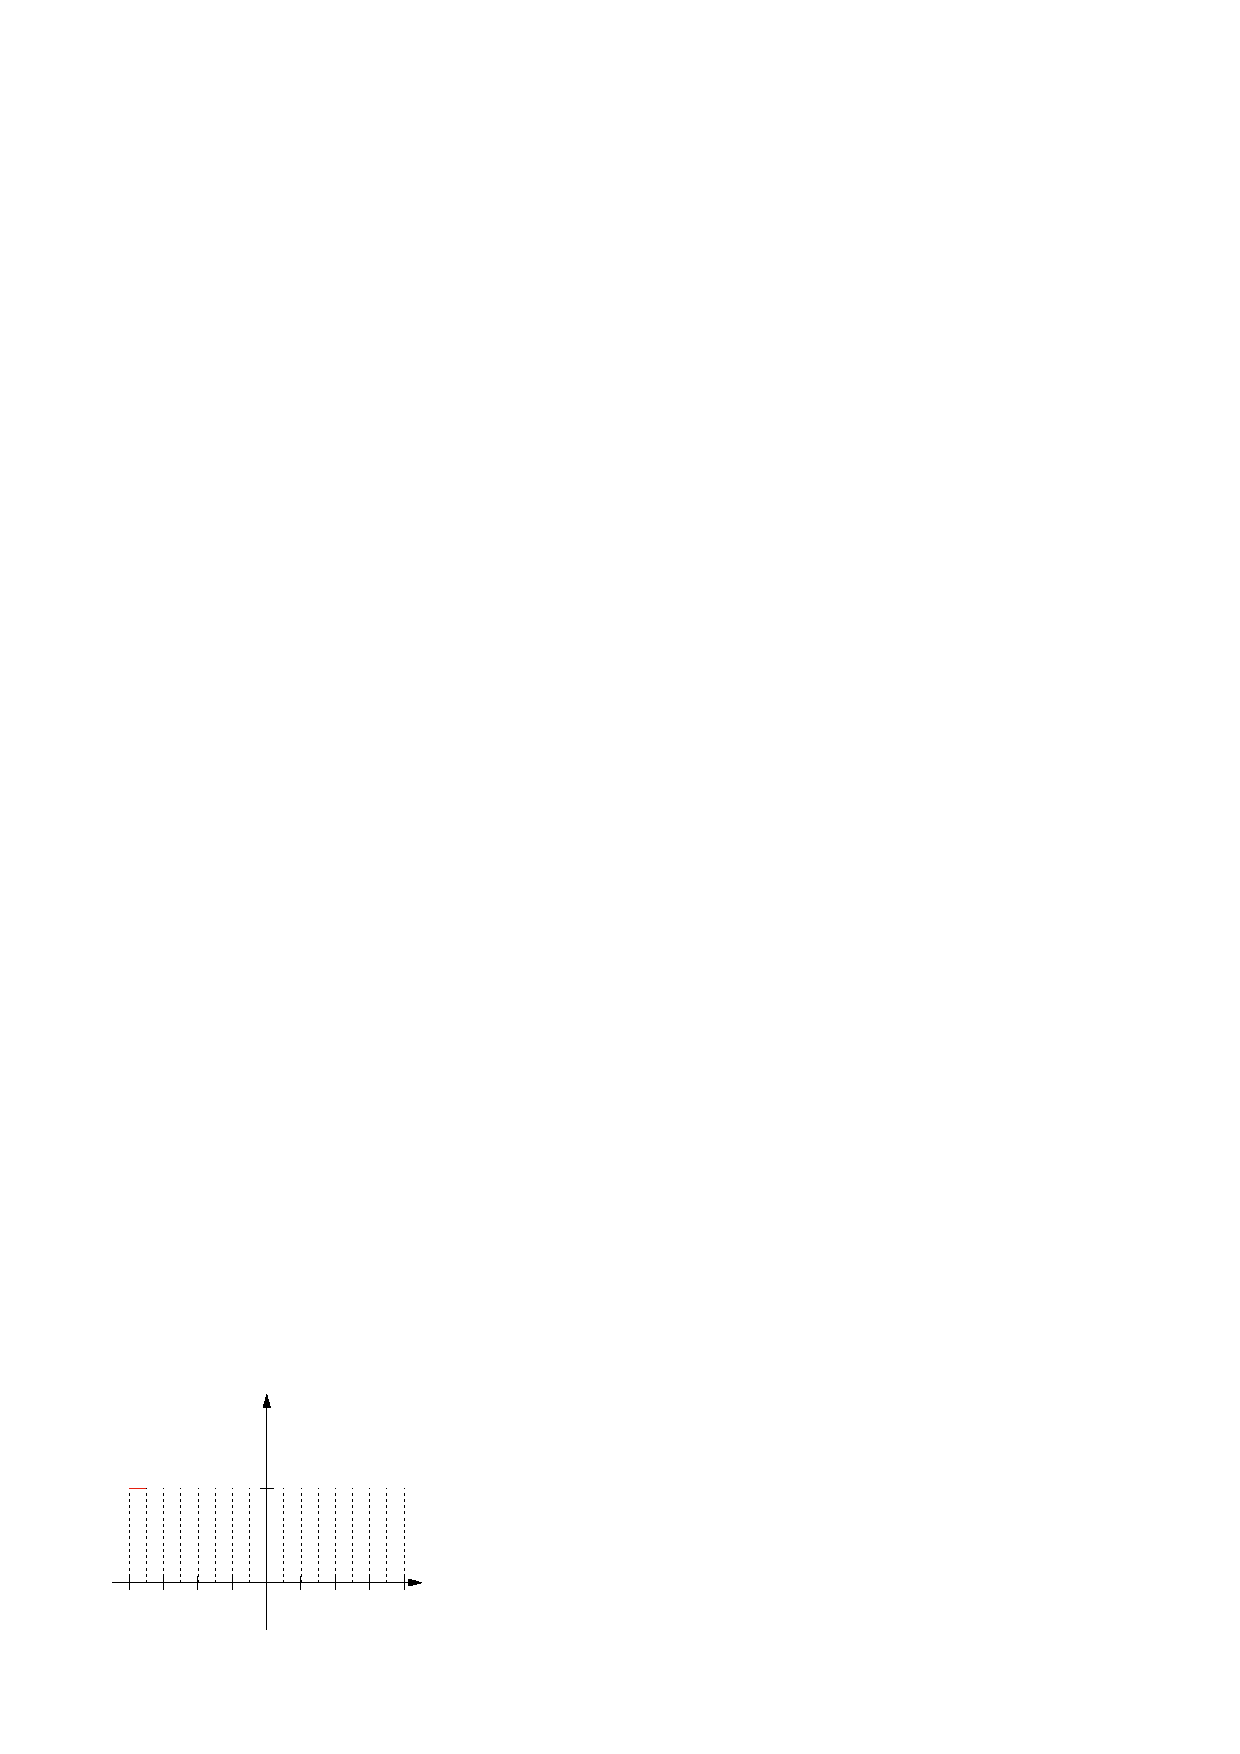
\includegraphics[width={158.40bp},height={108.00bp}]{figura_04_04}}%
    \gplfronttext
  \end{picture}%
\endgroup

    \end{minipage}
\end{figure}

\section{Propiedades de la transformada de \emph{Fourier}}
\subsection{Linealidad}
\begin{equation}
    \mathcal{F}\{a_1f_1(t)+a_2f_2(t)\}=a_1F_1(\omega)+a_2F_2(\omega)
\end{equation}

Donde:
\begin{equation*}
    F_1(\omega)=\mathcal{F}\{f_1(t)\}
\end{equation*}
\begin{equation*}
    F_2(\omega)=\mathcal{F}\{f_2(t)\}
\end{equation*}

\subsection{Cambio de escala}
Si $\mathcal{F}\{f(t)\}=F(\omega)$:
\begin{equation}
    \mathcal{F}\{f(at)\}=\frac{1}{|a|}F\left(\frac{\omega}{a}\right)
\end{equation}

\underline{Prueba}:

\begin{equation*}
    \mathcal{F}\{f(at)\}=\int_{-\infty}^\infty f(at)\,e^{-j\omega t}\,dt
\end{equation*}

Realizando un cambio de variable:
\begin{equation*}
    \tau=at
\end{equation*}
\begin{equation*}
    d\tau=a\,dt
\end{equation*}

Para $a>0$:
\begin{equation*}
\begin{split}
    \mathcal{F}\{f(at)\}
        &=\int_{-\infty}^\infty\,f(\tau)\,e^{-j\omega
            \frac{\tau}{a}}\,\frac{d\tau}{a}\\
        &=\frac{1}{a}\int_{-\infty}^\infty\,f(\tau)\,e^{-j\omega
            \frac{\tau}{a}}d\tau\\
        &=\frac{1}{a}F\left(\frac{\omega}{a}\right)\\
\end{split}
\end{equation*}

Para $a<0$:
\begin{equation*}
\begin{split}
    \mathcal{F}\{f(at)\}
        &=\int_\infty^{-\infty}f(\tau)\,e^{-j\omega
            \frac{\tau}{a}}\,\frac{d\tau}{a}\\
        &=-\frac{1}{a}\int_{-\infty}^\infty\,f(\tau)\,e^{-j\omega
            \frac{\tau}{a}}d\tau\\
        &=-\frac{1}{a}F\left(\frac{\omega}{a}\right)\\
\end{split}
\end{equation*}

\subsection{Desplazamiento en $\omega$}
Si $\mathcal{F}\{f(t)\}=F(\omega)$:
\begin{equation}
    \mathcal{F}\{f(t)\,e^{jat}\}=F(\omega-a)
\end{equation}

\underline{Prueba}:

\begin{equation*}
\begin{split}
    \mathcal{F}\{f(t)\,e^{jat}\}
        &=\int_{-\infty}^\infty\,f(t)\,e^{jat}\,e^{-j\omega\,t}\,dt\\
        &=\int_{-\infty}^\infty\,f(t)\,e^{-j(\omega-a)t}\,dt\\
        &=F(\omega-a)\\
\end{split}
\end{equation*}

\subsection{Desplazamiento en $t$}
Si $\mathcal{F}\{f(t)\}=F(\omega)$:
\begin{equation}
    \mathcal{F}\{f(t-a)\}=F(\omega)\,e^{-ja\omega}
\end{equation}

\underline{Prueba}:

\begin{equation*}
    \mathcal{F}\{f(t-a)\}=\int_{-\infty}^\infty\,f(t-a)\,e^{-j\omega\,t}\,dt
\end{equation*}

Realizando un cambio de variable:
\begin{equation*}
    \tau=t-a
\end{equation*}
\begin{equation*}
    d\tau=dt
\end{equation*}

\begin{equation*}
\begin{split}
    \mathcal{F}\{f(t-a)\}
        &=\int_{-\infty}^\infty\,f(\tau)\,e^{-j\omega(\tau+a)}\,dt\\
        &=e^{-ja\omega}\int_{-\infty}^\infty\,f(\tau)\,e^{-j\omega\tau}\,d\tau\\
        &=e^{-ja\omega}F(\omega)\\
\end{split}
\end{equation*}

\subsection{Simetría}
Si $\mathcal{F}\{f(t)\}=F(\omega)$:
\begin{equation}
    \mathcal{F}\{F(t)\}=2\pi\,f(-\omega)
\end{equation}

\underline{Prueba}:

\begin{equation*}
    f(t)=\frac{1}{2\pi}\int_{-\infty}^\infty\,F(\omega)\,e^{j\omega\,t}\,d\omega
\end{equation*}

Reemplazando:
\begin{equation*}
    t\to-\omega
\end{equation*}
\begin{equation*}
    \omega\to\,t
\end{equation*}

\begin{equation*}
\begin{split}
    f(-\omega)=
        &=\frac{1}{2\pi}\int_{-\infty}^\infty\,F(t)\,e^{jt(-\omega)}\,dt\\
        &=\frac{1}{2\pi}\mathcal{F}\{F(t)\}\\
\end{split}
\end{equation*}
\begin{equation*}
    2\pi\,f(-\omega)=\mathcal{F}\{F(t)\}
\end{equation*}

\textbf{Ejemplo 2:} Hallar $\mathcal{F}\biggl\{\dfrac{\sen(at)}{t}\biggl\}$
Sabiendo que:
\begin{equation*}
    \mathcal{F}\{u(t+a)-u(t-a)\}=\dfrac{2\sen(a\omega)}{\omega}
\end{equation*}
\begin{equation*}
    \mathcal{F}\biggl\{\dfrac{2\sen(at)}{t}\biggl\}=2\pi(u(t+a)-u(t-a))
\end{equation*}
\begin{equation}
    \mathcal{F}\biggl\{\dfrac{\sen(at)}{t}\biggl\}=\pi(u(t+a)-u(t-a))
\end{equation}

\subsection{Multiplicación por $t$}
Si $\mathcal{F}\{f(t)\}=F(\omega)$:
\begin{equation*}
    \mathcal{F}\{t\,f(t)\}=j\frac{dF(\omega)}{d\omega}
\end{equation*}

En general:
\begin{equation}
    \mathcal{F}\{t^n\,f(t)\}=j^n\frac{d^{(n)}F(\omega)}{d\omega^n};
    \quad\,n\in\mathbb{N}
\end{equation}

\underline{Prueba}:

\begin{equation*}
    F(\omega)=\int_{-\infty}^\infty\,f(t)\,e^{-j\omega\,t}\,dt
\end{equation*}

\begin{equation*}
\begin{split}
    \frac{dF(\omega)}{d\omega}
        &=\int_{-\infty}^\infty\,f(t)\,e^{-j\omega\,t}(-jt)\,dt\\
        &=-j\int_{-\infty}^\infty\,t\,f(t)\,e^{-j\omega\,t}\,dt\\
        &=-j\,\mathcal{F}\{t\,f(t)\}\\
\end{split}
\end{equation*}
\begin{equation*}
    j\frac{dF(\omega)}{d\omega}=\mathcal{F}\{t\,f(t)\}
\end{equation*}
\begin{equation*}
\begin{split}
    \mathcal{F}\{t^2\,f(t)\}
        &=\mathcal{F}\{t\,t\,f(t)\}\\
        &=j\frac{d}{d\omega}\left(\mathcal{F}\{t\,f(t)\}\right)\\
        &=j\frac{d}{d\omega}\left(j\frac{dF(\omega)}{d\omega}\right)\\
        &=j^2\frac{d^2F(\omega)}{d\omega^2}\\
\end{split}
\end{equation*}
\begin{equation*}
    \mathcal{F}\{t^n\,f(t)\}=j^n\frac{d^{(n)}\,F(\omega)}{d\omega^n}\\
\end{equation*}

\textbf{Ejemplo 3:} Hallar $\mathcal{F}\{t^n\,e^{-at}\,u(t)\};
\quad\,n\in\mathbb{N}$

Para $n=1$:
\begin{equation*}
\begin{split}
    \mathcal{F}\{t\,e^{-at}\,u(t)\}
        &=j\frac{d}{d\omega}\left(\frac{1}{a+j\omega}\right)\\
        &=(j)(-1){(a+j\omega)}^{-2}(j)\\
        &=\frac{1}{{(a+j\omega)}^2}\\
\end{split}
\end{equation*}

Para $n=2$:
\begin{equation*}
\begin{split}
    \mathcal{F}\{t^2\,e^{-at}\,u(t)\}
        &=j\frac{d}{d\omega}\left(\frac{1}{{(a+j\omega)}^2}\right)\\
        &=(j)(-2){(a+j\omega)}^{-3}(j)\\
        &=\frac{2}{{(a+j\omega)}^3}\\
\end{split}
\end{equation*}

Para $n=3$:
\begin{equation*}
\begin{split}
    \mathcal{F}\{t^3\,e^{-at}\,u(t)\}
        &=j\frac{d}{d\omega}\left(\frac{2}{{(a+j\omega)}^3}\right)\\
        &=(j)(2)(-3){(a+j\omega)}^{-4}(j)\\
        &=\frac{6}{{(a+j\omega)}^4}\\
\end{split}
\end{equation*}

Por tanto:
\begin{equation}
    \mathcal{F}\{t^n\,e^{-at}\,u(t)\}=\frac{n!}{{(a+j\omega)}^{n+1}}
\end{equation}

\subsection{Transformada de \emph{Fourier} de una derivada}
Si $\mathcal{F}\{f(t)\}=F(\omega)$:
\begin{equation*}
    \mathcal{F}\{f'(t)\}=j\omega\,F(\omega)
\end{equation*}

En general:
\begin{equation}
    \mathcal{F}\{f^{(n)}(t)\}={(j\omega)}^n\,F(\omega)
    \quad\,n\in\mathbb{N}
\end{equation}

\underline{Prueba}:

\begin{equation*}
    \mathcal{F}\{f'(t)\}=\int_{\infty}^\infty\,f'(t)\,e^{-j\omega\,t}\,dt
\end{equation*}

Realizando la integración por partes:
\begin{equation*}
    u=e^{-j\omega\,t}
\end{equation*}
\begin{equation*}
    du=-j\omega\,e^{-j\omega\,t}\,dt
\end{equation*}
\begin{equation*}
    dv=f'(t)\,dt
\end{equation*}
\begin{equation*}
    v=f(t)
\end{equation*}
\begin{equation*}
    \mathcal{F}\{f'(t)\}
        =\left(f(t)\,e^{-j\omega\,t}\Biggr|_{-\infty}^\infty\right)
        -\int_{-\infty}^\infty\,f(t)\,(-j\omega\,e^{-j\omega\,t})\,dt
\end{equation*}

Asumiendo $f(\pm\infty)=0$:
\begin{equation*}
\begin{split}
    \mathcal{F}\{f'(t)\}
        &=j\omega\int_{-\infty}^\infty\,f(t)\,e^{-j\omega\,t}\,dt\\
        &=j\omega\,F(\omega)\\
\end{split}
\end{equation*}

Para la segunda derivada:
\begin{equation*}
\begin{split}
    \mathcal{F}\{f^{\prime\prime}(t)\}
        &=\mathcal{F}\{(f'(t))'\}\\
        &=j\omega\,\mathcal{F}\{f'(t)\}\\
        &=j\omega(j\omega\,F(\omega))\\
        &={(j\omega)}^2\,F(\omega)\\
\end{split}
\end{equation*}

Por tanto:
\begin{equation*}
    \mathcal{F}\{f^{(n)}(t)\}={(j\omega)}^n\,F(\omega)
\end{equation*}

\section{Transformadas de \emph{Fourier} especiales}
\subsection{$e^{-at}\,u(t);\quad\,a>0$}
\begin{equation*}
    \mathcal{F}\{e^{-at}\,u(t)\};a>0
\end{equation*}
\begin{equation*}
\begin{split}
    \mathcal{F}\{e^{-at}\,u(t)\}
        &=\int_0^\infty\,e^{-at}\,e^{-j\omega\,t}\,dt\\
        &=\int_0^\infty\,e^{-(a+j\omega)t}\,dt\\
        &=\frac{e^{-(a+j\omega)t}}{-(a+j\omega)}\Biggr|_0^\infty\\
        &=\frac{0-1}{-(a+j\omega)}\\
        &=\frac{1}{a+j\omega}\\
\end{split}
\end{equation*}
\begin{equation}
    \mathcal{F}\{e^{-at}\,u(t)\}=\frac{1}{a+j\omega}\\
\end{equation}

\subsection{$e^{at}\,u(-t);\quad\,a>0$}
\begin{equation*}
    \mathcal{F}\{e^{at}\,u(-t)\};a>0
\end{equation*}
\begin{equation*}
\begin{split}
    \mathcal{F}\{e^{at}\,u(t)\}
        &=\int_{-\infty}^0\,e^{at}\,e^{-j\omega\,t}\,dt\\
        &=\int_{-\infty}^0\,e^{(a-j\omega)t}\,dt\\
        &=\frac{e^{(a-j\omega)t}}{a-j\omega}\Biggr|_{-\infty}^0\\
        &=\frac{1}{a-j\omega}\\
\end{split}
\end{equation*}
\begin{equation}
    \mathcal{F}\{e^{at}\,u(-t)\}=\frac{1}{a-j\omega}\\
\end{equation}

\subsection{$e^{-a|t|}$}
\begin{equation*}
    \mathcal{F}\{e^{-a|t|}\}
\end{equation*}
\begin{equation*}
\begin{split}
    \mathcal{F}\{e^{-a|t|}\}
        &=\mathcal{F}\{e^{at}u(-t)+e^{-at}u(t)\}\\
        &=\frac{1}{a-j\omega}+\frac{1}{a+j\omega}\\
        &=\frac{a+j\omega+a-j\omega}{(a-j\omega)(a+j\omega)}\\
        &=\frac{2a}{a^2+\omega^2}
\end{split}
\end{equation*}
\begin{equation}
    \mathcal{F}\{e^{-a|t|}\}=\frac{2a}{a^2+\omega^2}
\end{equation}

\subsection{$\delta(t-t_0)$}
\begin{equation*}
    \mathcal{F}\{\delta(t-t_0)\}
\end{equation*}
\begin{equation*}
\begin{split}
    \mathcal{F}\{\delta(t-t_0)\}
        &=\int_{-\infty}^0\delta(t-t_0)\,e^{-j\omega\,t}\,dt\\
        &=e^{-j\omega\,t_0}\\
\end{split}
\end{equation*}
\begin{equation}
    \mathcal{F}\{\delta(t-t_0)\}=e^{-j\omega\,t_0}
\end{equation}

En particular:
\begin{equation*}
    \mathcal{F}\{\delta(t)\}=1
\end{equation*}

\subsection{$e^{jat}$}
Sabiendo:
\begin{equation*}
    \mathcal{F}\{\delta(t-a)\}=e^{-ja\omega}
\end{equation*}

Aplicando la propiedad de simetría:
\begin{equation*}
    \mathcal{F}\{e^{-jat}\}=2\pi\delta(-\omega-a)\
\end{equation*}
\begin{equation*}
\begin{split}
    \mathcal{F}\{e^{jat}\}
        &=2\pi\delta(-\omega+a)\\
        &=2\pi\delta(-(\omega-a))\\
        &=2\pi\delta(\omega-a)\\
\end{split}
\end{equation*}
\begin{equation}
    \mathcal{F}\{e^{jat}\}=2\pi\delta(\omega-a)
\end{equation}

En particular:
\begin{equation*}
    \mathcal{F}\{1\}=2\pi\delta(\omega)
\end{equation*}
\begin{equation*}
    \mathcal{F}\{k\}=2\pi\,k\delta(\omega)
\end{equation*}

\subsection{$\sen(at)$}
\begin{equation*}
\begin{split}
    \mathcal{F}\{\sen(at)\}
        &=\mathcal{F}\biggl\{\frac{e^{jat}-e^{-jat}}{2j}\biggl\}\\
        &=\frac{1}{2j}\left(2\pi\delta(\omega-a)-2\pi\delta(\omega+a)\right)\\
        &=-j\pi(\delta(\omega-a)-\delta(\omega+a))
\end{split}
\end{equation*}
\begin{equation}
    \mathcal{F}\{\sen(at)\}=j\pi(\delta(\omega+a)+\delta(\omega-a))
\end{equation}

\subsection{$\cos(at)$}
\begin{equation*}
\begin{split}
    \mathcal{F}\{\cos(at)\}
        &=\mathcal{F}\biggl\{\frac{e^{jat}+e^{-jat}}{2}\biggl\}\\
        &=\frac{1}{2}\left(2\pi\delta(\omega-a)+2\pi\delta(\omega+a)\right)\\
        &=\pi(\delta(\omega+a)+\delta(\omega-a))
\end{split}
\end{equation*}
\begin{equation}
    \mathcal{F}\{\cos(at)\}=\pi(\delta(\omega+a)+\delta(\omega-a))
\end{equation}

\subsection{$u(t)$}
\begin{equation*}
    u(t)+u(-t)=1
\end{equation*}
\begin{equation*}
    \mathcal{F}\{u(t)+u(-t)\}=\mathcal{F}\{1\}
\end{equation*}

Considerando:
\begin{equation*}
    \mathcal{F}\{u(t)\}=F(\omega)
\end{equation*}
\begin{equation*}
    \mathcal{F}\{u(-t)\}=F(-\omega)
\end{equation*}

Por tanto:
\begin{equation*}
    F(\omega)+F(-\omega)=2\pi\delta(\omega)
\end{equation*}

Se asume que la transformada de \emph{Fourier} de la función escalón tendrá un
termino impulsivo:
\begin{equation*}
    F(\omega)=\beta(\omega)+k\delta(\omega)
\end{equation*}
\begin{equation*}
    F(-\omega)=\beta(-\omega)+k\delta(\omega)
\end{equation*}
\begin{equation*}
    F(\omega)+F(-\omega)=\beta(\omega)+\beta(-\omega)+2k\delta(\omega)
\end{equation*}

Reemplazando:
\begin{equation*}
    \beta(\omega)+\beta(-\omega)+2k\delta(\omega)=2\pi\delta(\omega)
\end{equation*}

Por tanto:
\begin{equation*}
    k=\pi
\end{equation*}

Resultando:
\begin{equation*}
    F(\omega)=\beta(\omega)+\pi\delta(\omega)
\end{equation*}

Por otro lado, se sabe que:
\begin{equation*}
    u'(t)=\delta(t)
\end{equation*}
\begin{equation*}
    \mathcal{F}\{u'(t)\}=\mathcal{F}\{\delta(t)\}
\end{equation*}
\begin{equation*}
    j\omega\mathcal{F}\{u(t)\}=1
\end{equation*}
\begin{equation*}
    j\omega(\beta(\omega)+\pi\delta(\omega))=1
\end{equation*}
\begin{equation*}
    j\omega\beta(\omega)+j\pi\omega\delta(\omega)=1
\end{equation*}
\begin{equation*}
    j\omega\beta(\omega)=1
\end{equation*}
\begin{equation*}
    \beta(\omega)=\frac{1}{j\omega}
\end{equation*}
\begin{equation}
    \mathcal{F}\{u(t)\}=\frac{1}{j\omega}+\pi\delta(\omega)
\end{equation}

\section{La función signo}
\begin{equation}
    \sgn(t)=\begin{cases}
        -1&t<0\\
        1&t>0\\
    \end{cases}
\end{equation}
\begin{figure}[H]
    \centering
    % GNUPLOT: LaTeX picture with Postscript
\begingroup
  \makeatletter
  \providecommand\color[2][]{%
    \GenericError{(gnuplot) \space\space\space\@spaces}{%
      Package color not loaded in conjunction with
      terminal option `colourtext'%
    }{See the gnuplot documentation for explanation.%
    }{Either use 'blacktext' in gnuplot or load the package
      color.sty in LaTeX.}%
    \renewcommand\color[2][]{}%
  }%
  \providecommand\includegraphics[2][]{%
    \GenericError{(gnuplot) \space\space\space\@spaces}{%
      Package graphicx or graphics not loaded%
    }{See the gnuplot documentation for explanation.%
    }{The gnuplot epslatex terminal needs graphicx.sty or graphics.sty.}%
    \renewcommand\includegraphics[2][]{}%
  }%
  \providecommand\rotatebox[2]{#2}%
  \@ifundefined{ifGPcolor}{%
    \newif\ifGPcolor
    \GPcolorfalse
  }{}%
  \@ifundefined{ifGPblacktext}{%
    \newif\ifGPblacktext
    \GPblacktexttrue
  }{}%
  % define a \g@addto@macro without @ in the name:
  \let\gplgaddtomacro\g@addto@macro
  % define empty templates for all commands taking text:
  \gdef\gplbacktext{}%
  \gdef\gplfronttext{}%
  \makeatother
  \ifGPblacktext
    % no textcolor at all
    \def\colorrgb#1{}%
    \def\colorgray#1{}%
  \else
    % gray or color?
    \ifGPcolor
      \def\colorrgb#1{\color[rgb]{#1}}%
      \def\colorgray#1{\color[gray]{#1}}%
      \expandafter\def\csname LTw\endcsname{\color{white}}%
      \expandafter\def\csname LTb\endcsname{\color{black}}%
      \expandafter\def\csname LTa\endcsname{\color{black}}%
      \expandafter\def\csname LT0\endcsname{\color[rgb]{1,0,0}}%
      \expandafter\def\csname LT1\endcsname{\color[rgb]{0,1,0}}%
      \expandafter\def\csname LT2\endcsname{\color[rgb]{0,0,1}}%
      \expandafter\def\csname LT3\endcsname{\color[rgb]{1,0,1}}%
      \expandafter\def\csname LT4\endcsname{\color[rgb]{0,1,1}}%
      \expandafter\def\csname LT5\endcsname{\color[rgb]{1,1,0}}%
      \expandafter\def\csname LT6\endcsname{\color[rgb]{0,0,0}}%
      \expandafter\def\csname LT7\endcsname{\color[rgb]{1,0.3,0}}%
      \expandafter\def\csname LT8\endcsname{\color[rgb]{0.5,0.5,0.5}}%
    \else
      % gray
      \def\colorrgb#1{\color{black}}%
      \def\colorgray#1{\color[gray]{#1}}%
      \expandafter\def\csname LTw\endcsname{\color{white}}%
      \expandafter\def\csname LTb\endcsname{\color{black}}%
      \expandafter\def\csname LTa\endcsname{\color{black}}%
      \expandafter\def\csname LT0\endcsname{\color{black}}%
      \expandafter\def\csname LT1\endcsname{\color{black}}%
      \expandafter\def\csname LT2\endcsname{\color{black}}%
      \expandafter\def\csname LT3\endcsname{\color{black}}%
      \expandafter\def\csname LT4\endcsname{\color{black}}%
      \expandafter\def\csname LT5\endcsname{\color{black}}%
      \expandafter\def\csname LT6\endcsname{\color{black}}%
      \expandafter\def\csname LT7\endcsname{\color{black}}%
      \expandafter\def\csname LT8\endcsname{\color{black}}%
    \fi
  \fi
    \setlength{\unitlength}{0.0500bp}%
    \ifx\gptboxheight\undefined%
      \newlength{\gptboxheight}%
      \newlength{\gptboxwidth}%
      \newsavebox{\gptboxtext}%
    \fi%
    \setlength{\fboxrule}{0.5pt}%
    \setlength{\fboxsep}{1pt}%
    \definecolor{tbcol}{rgb}{1,1,1}%
\begin{picture}(4320.00,2014.00)%
    \gplgaddtomacro\gplbacktext{%
      \csname LTb\endcsname%%
      \put(2040,469){\makebox(0,0)[r]{\strut{}}}%
      \put(2040,1023){\makebox(0,0)[r]{\strut{}}}%
      \put(2040,1576){\makebox(0,0)[r]{\strut{}}}%
      \put(240,800){\makebox(0,0){\strut{}}}%
      \put(619,800){\makebox(0,0){\strut{}}}%
      \put(998,800){\makebox(0,0){\strut{}}}%
      \put(1377,800){\makebox(0,0){\strut{}}}%
      \put(1756,800){\makebox(0,0){\strut{}}}%
      \put(2136,800){\makebox(0,0){\strut{}}}%
      \put(2515,800){\makebox(0,0){\strut{}}}%
      \put(2894,800){\makebox(0,0){\strut{}}}%
      \put(3273,800){\makebox(0,0){\strut{}}}%
      \put(3652,800){\makebox(0,0){\strut{}}}%
      \put(4031,800){\makebox(0,0){\strut{}}}%
      \csname LTb\endcsname%%
      \put(4600,1023){\makebox(0,0)[l]{\strut{}$t$}}%
      \put(2325,1798){\makebox(0,0)[l]{\strut{}$f(t)$}}%
      \put(1946,1576){\makebox(0,0)[l]{\strut{}$1$}}%
      \put(2287,469){\makebox(0,0)[l]{\strut{}$-1$}}%
    }%
    \gplgaddtomacro\gplfronttext{%
    }%
    \gplgaddtomacro\gplbacktext{%
      \csname LTb\endcsname%%
      \put(2040,469){\makebox(0,0)[r]{\strut{}}}%
      \put(2040,1023){\makebox(0,0)[r]{\strut{}}}%
      \put(2040,1576){\makebox(0,0)[r]{\strut{}}}%
      \put(240,800){\makebox(0,0){\strut{}}}%
      \put(619,800){\makebox(0,0){\strut{}}}%
      \put(998,800){\makebox(0,0){\strut{}}}%
      \put(1377,800){\makebox(0,0){\strut{}}}%
      \put(1756,800){\makebox(0,0){\strut{}}}%
      \put(2136,800){\makebox(0,0){\strut{}}}%
      \put(2515,800){\makebox(0,0){\strut{}}}%
      \put(2894,800){\makebox(0,0){\strut{}}}%
      \put(3273,800){\makebox(0,0){\strut{}}}%
      \put(3652,800){\makebox(0,0){\strut{}}}%
      \put(4031,800){\makebox(0,0){\strut{}}}%
      \csname LTb\endcsname%%
      \put(4600,1023){\makebox(0,0)[l]{\strut{}$t$}}%
      \put(2325,1798){\makebox(0,0)[l]{\strut{}$f(t)$}}%
      \put(1946,1576){\makebox(0,0)[l]{\strut{}$1$}}%
      \put(2287,469){\makebox(0,0)[l]{\strut{}$-1$}}%
    }%
    \gplgaddtomacro\gplfronttext{%
    }%
    \gplbacktext
    \put(0,0){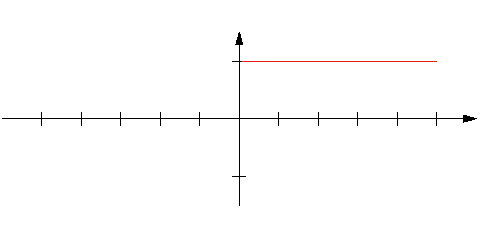
\includegraphics[width={216.00bp},height={100.70bp}]{figura_04_05}}%
    \gplfronttext
  \end{picture}%
\endgroup

\end{figure}

Esta función puede representarse también como:
\begin{equation*}
    \sgn(t)=\frac{|t|}{t}
\end{equation*}
\begin{equation*}
    \sgn(t)=-1+2u(t)
\end{equation*}

A partir de la definición de la función de valor absoluto:
\begin{equation*}
    |t|=\begin{cases}
        -t&t<0\\
        t&t>0\\
    \end{cases}
\end{equation*}

Es posible calcular la derivada del valor absoluto:
\begin{equation*}
    |t|'=\begin{cases}
        -1&t<0\\
        1&t>0\\
    \end{cases}
\end{equation*}

Por tanto:
\begin{equation}
    |t|'=\sgn(t)
\end{equation}

Cuya derivada es:
\begin{equation}
    \sgn'(t)=2\delta(t)
\end{equation}

Calculando su transformada de \emph{Fourier}:
\begin{equation*}
\begin{split}
    \mathcal{F}\{\sgn(t)\}
        &=\mathcal{F}\{-1+2u(t)\}\\
        &=-2\pi\delta(\omega)
            +2\left(\frac{1}{j\omega}+\pi\delta(\omega)\right)\\
        &=-2\pi\delta(\omega)
            +2\left(\frac{1}{j\omega}\right)+2\pi\delta(\omega)\\
        &=\frac{2}{j\omega}
\end{split}
\end{equation*}
\begin{equation}
    \mathcal{F}\{\sgn(t)\}=\frac{2}{j\omega}
\end{equation}

\subsection{Transformada de \emph{Fourier} de $|t|$}
\begin{equation*}
    \mathcal{F}\{|t|'\}=\mathcal{F}\{\sgn(t)\}
\end{equation*}
\begin{equation*}
    j\omega\mathcal{F}\{|t|\}=\frac{2}{j\omega}
\end{equation*}
\begin{equation}
    \mathcal{F}\{|t|\}=-\frac{2}{j\omega^2}
\end{equation}

\subsection{Transformada de \emph{Fourier} de $1/t$}
\begin{equation*}
    \mathcal{F}\{\sgn(t)\}=\frac{2}{j\omega}
\end{equation*}

Por simetría:
\begin{equation*}
    \mathcal{F}\biggl\{\frac{2}{jt}\biggl\}=2\pi\,\sgn(-\omega)
\end{equation*}
\begin{equation}
    \mathcal{F}\biggl\{\frac{1}{t}\biggl\}=-j\pi\,\sgn(-\omega)
\end{equation}

Calculando la segunda derivada:
\begin{equation*}
    \left(\frac{1}{t}\right)'=-\frac{1}{t^2}
\end{equation*}
\begin{equation*}
    \mathcal{F}\biggl\{-\frac{1}{t^2}\biggl\}=j\omega(-j\pi\,\sgn(\omega))
\end{equation*}
\begin{equation*}
    \mathcal{F}\biggl\{-\frac{1}{t^2}\biggl\}=j^2\pi\omega\,\sgn(\omega)
\end{equation*}

Calculando la derivada n-ésima:
\begin{equation*}
    {\left(\frac{1}{t}\right)}^{\prime\prime}=\frac{2}{t^3}
\end{equation*}
\begin{equation*}
    {\left(\frac{1}{t}\right)}^{\prime\prime\prime}=-\frac{6}{t^4}
\end{equation*}
\begin{equation*}
    {\left(\frac{1}{t}\right)}^{(n)}={(-1)}^k\frac{k!}{t^{k+1}}
\end{equation*}
\begin{equation*}
    \mathcal{F}\{f^{(k)}(t)\}={(-1)}^k\,k!\,\mathcal{F}\biggl\{\frac{1}{t^{k+1}}\biggl\}
\end{equation*}
\begin{equation*}
    {(j\omega)}^k(-j\pi\,\sgn(\omega))={(-1)}^k\,k!\,\mathcal{F}\biggl\{\frac{1}{t^{k+1}}\biggl\}
\end{equation*}
\begin{equation*}
    -j^{k+1}\pi\omega^k\,\sgn(\omega)={(-1)}^k\,k!\,\mathcal{F}\biggl\{\frac{1}{t^{k+1}}\biggl\}
\end{equation*}
\begin{equation*}
    -j^n\pi\omega^{n-1}\,\sgn(\omega)={(-1)}^{n-1}\,(n-1)!\,\mathcal{F}\biggl\{\frac{1}{t^n}\biggl\}
\end{equation*}
\begin{equation*}
    -j^n\pi\omega^{n-1}\,\sgn(\omega)={(-1)}^n{(-1)}^{-1}(n-1)!\mathcal{F}\biggl\{\frac{1}{t^n}\biggl\}
\end{equation*}
\begin{equation}
    \mathcal{F}\biggl\{\frac{1}{t^n}\biggl\}=\frac{j^n\pi{\omega}^{n-1}\,\sgn(\omega)}{{(-1)}^n(n-1)!}
\end{equation}

\section{Tabla de transformadas de \emph{Fourier} conocidas}

\begin{equation*}
\def\arraystretch{1.4}
\begin{array}{@{}cll@{}}
\toprule
 & f(t) & F(\omega)=\mathcal{F}\{f(t)\}\\
\cmidrule(l){1-3}
 1 & u(t+a)-u(t-a)
   & \dfrac{2\sen(a\omega)}{\omega}\\
\cmidrule(l){1-3}
 2 & \dfrac{\sen(at)}{t}
   & \pi[u(\omega+a)-u(\omega-a)]\\
\cmidrule(l){1-3}
 3 & e^{-at}\,u(t)\quad\,a>0
   & \dfrac{1}{a+j\omega}\\
\cmidrule(l){1-3}
 4 & e^{at}\,u(-t)\quad\,a>0
   & \dfrac{1}{a-j\omega}\\
\cmidrule(l){1-3}
 5 & e^{-a|t|}\quad\,a>0
   & \dfrac{2a}{a^2+\omega^2}\\
\cmidrule(l){1-3}
 6 & \dfrac{1}{t^2+a^2}
   & \dfrac{\pi}{a}e^{-a|\omega|}\\
\cmidrule(l){1-3}
 7 & \delta(t-a)
   & e^{-ja\omega}\\
\cmidrule(l){1-3}
 8 & e^{jat}
   & 2\pi\delta(\omega-a)\\
\cmidrule(l){1-3}
 9 & k
   & 2\pi\,k\delta(\omega)\\
\cmidrule(l){1-3}
10 & \sen(at)
   & j\omega[\delta(\omega+a)-\delta(\omega-a)]\\
\cmidrule(l){1-3}
11 & \cos(at)
   & \pi[\delta(\omega+a)+\delta(\omega-a)]\\
\cmidrule(l){1-3}
12 & t^n\,e^{-at}\,u(t)
   & \dfrac{n!}{{(a+j\omega)}^{n+1}}\quad\,n\in\mathbb{N}\\
\cmidrule(l){1-3}
13 & u(t)
   & \dfrac{1}{j\omega}+\pi\delta(\omega)\\
\cmidrule(l){1-3}
14 & \sgn(t)
   & \dfrac{2}{j\omega}\\
\cmidrule(l){1-3}
15 & |t|
   & -\dfrac{2}{\omega^2}\\
\cmidrule(l){1-3}
16 & \dfrac{1}{t}
   & -j\pi\,\sgn(\omega)\\
\cmidrule(l){1-3}
17 & \dfrac{1}{t^n}
   & \dfrac{j^n\pi{\omega}^{n-1}\,\sgn(\omega)}{{(-1)}^n(n-1)!}\\
\bottomrule
\end{array}
\end{equation*}

